\subsection{Algorithm sketch}
\setlength{\unitlength}{0.8cm}
  \begin{figure}[H]
  \centering
  \begin{minipage}[!hp]{0.45\linewidth}
  \centering
    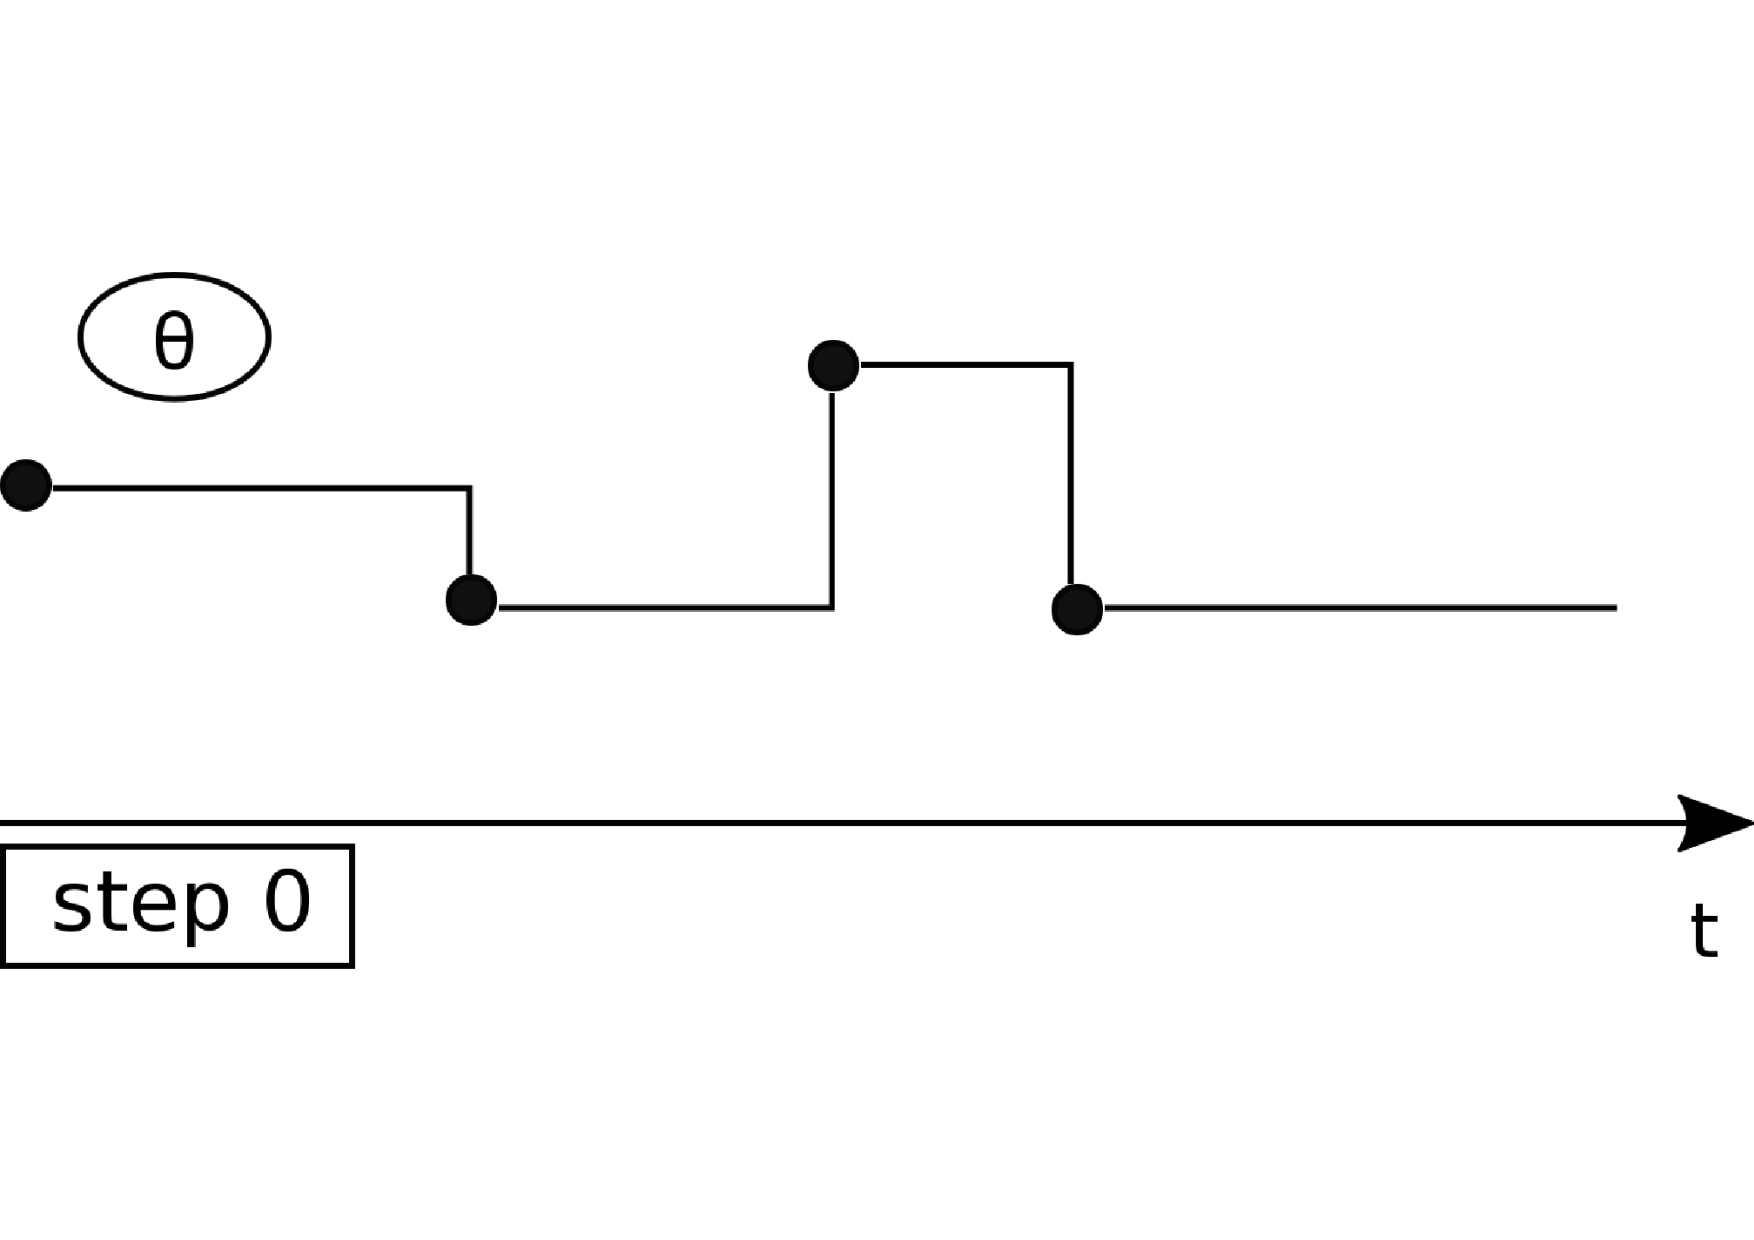
\includegraphics [width=0.70\textwidth, angle=0]{figs/plotn0.pdf}
      \end{minipage}
  \begin{minipage}[!hp]{0.45\linewidth}
  \centering
    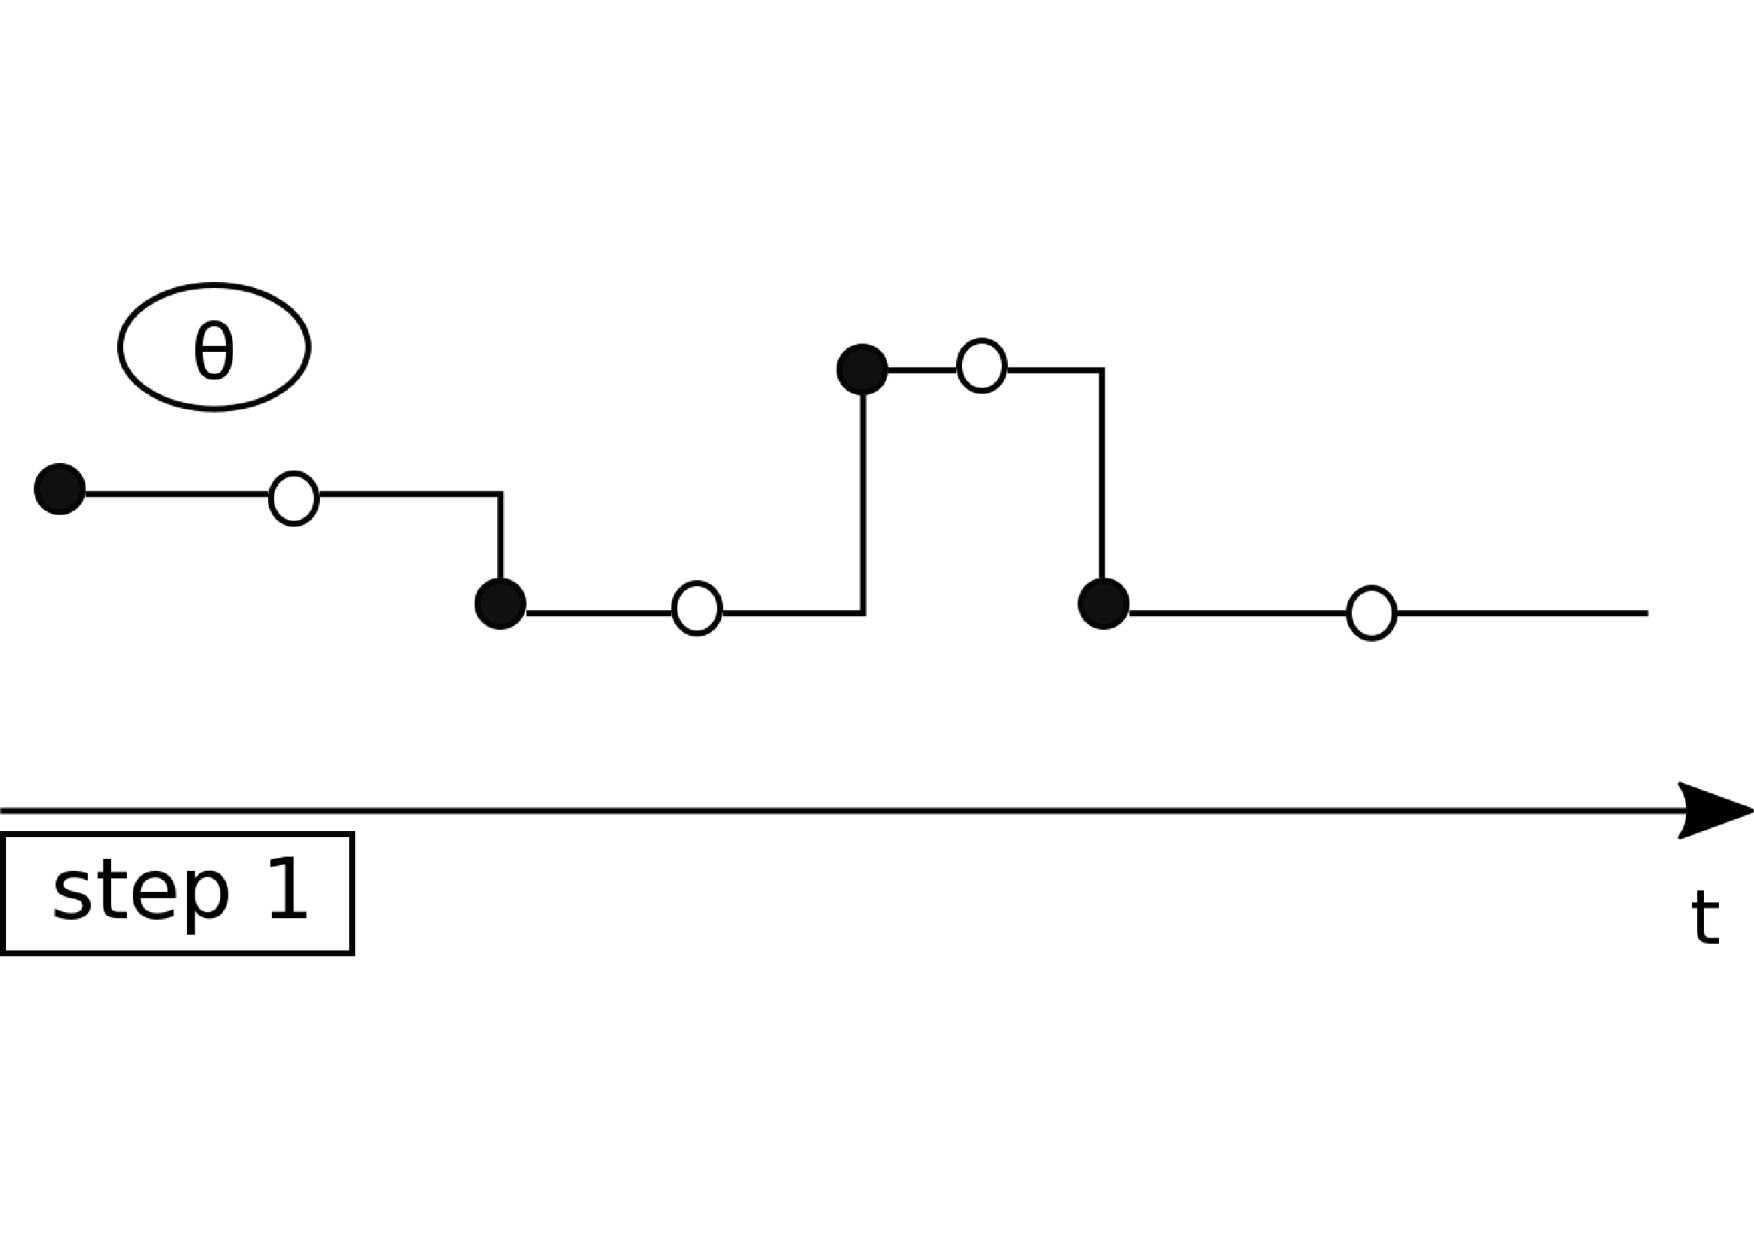
\includegraphics [width=0.70\textwidth, angle=0]{figs/plotn1.pdf}
    \vspace{-0 in}
  \end{minipage}
  \begin{minipage}[!hp]{0.45\linewidth}
  \centering
    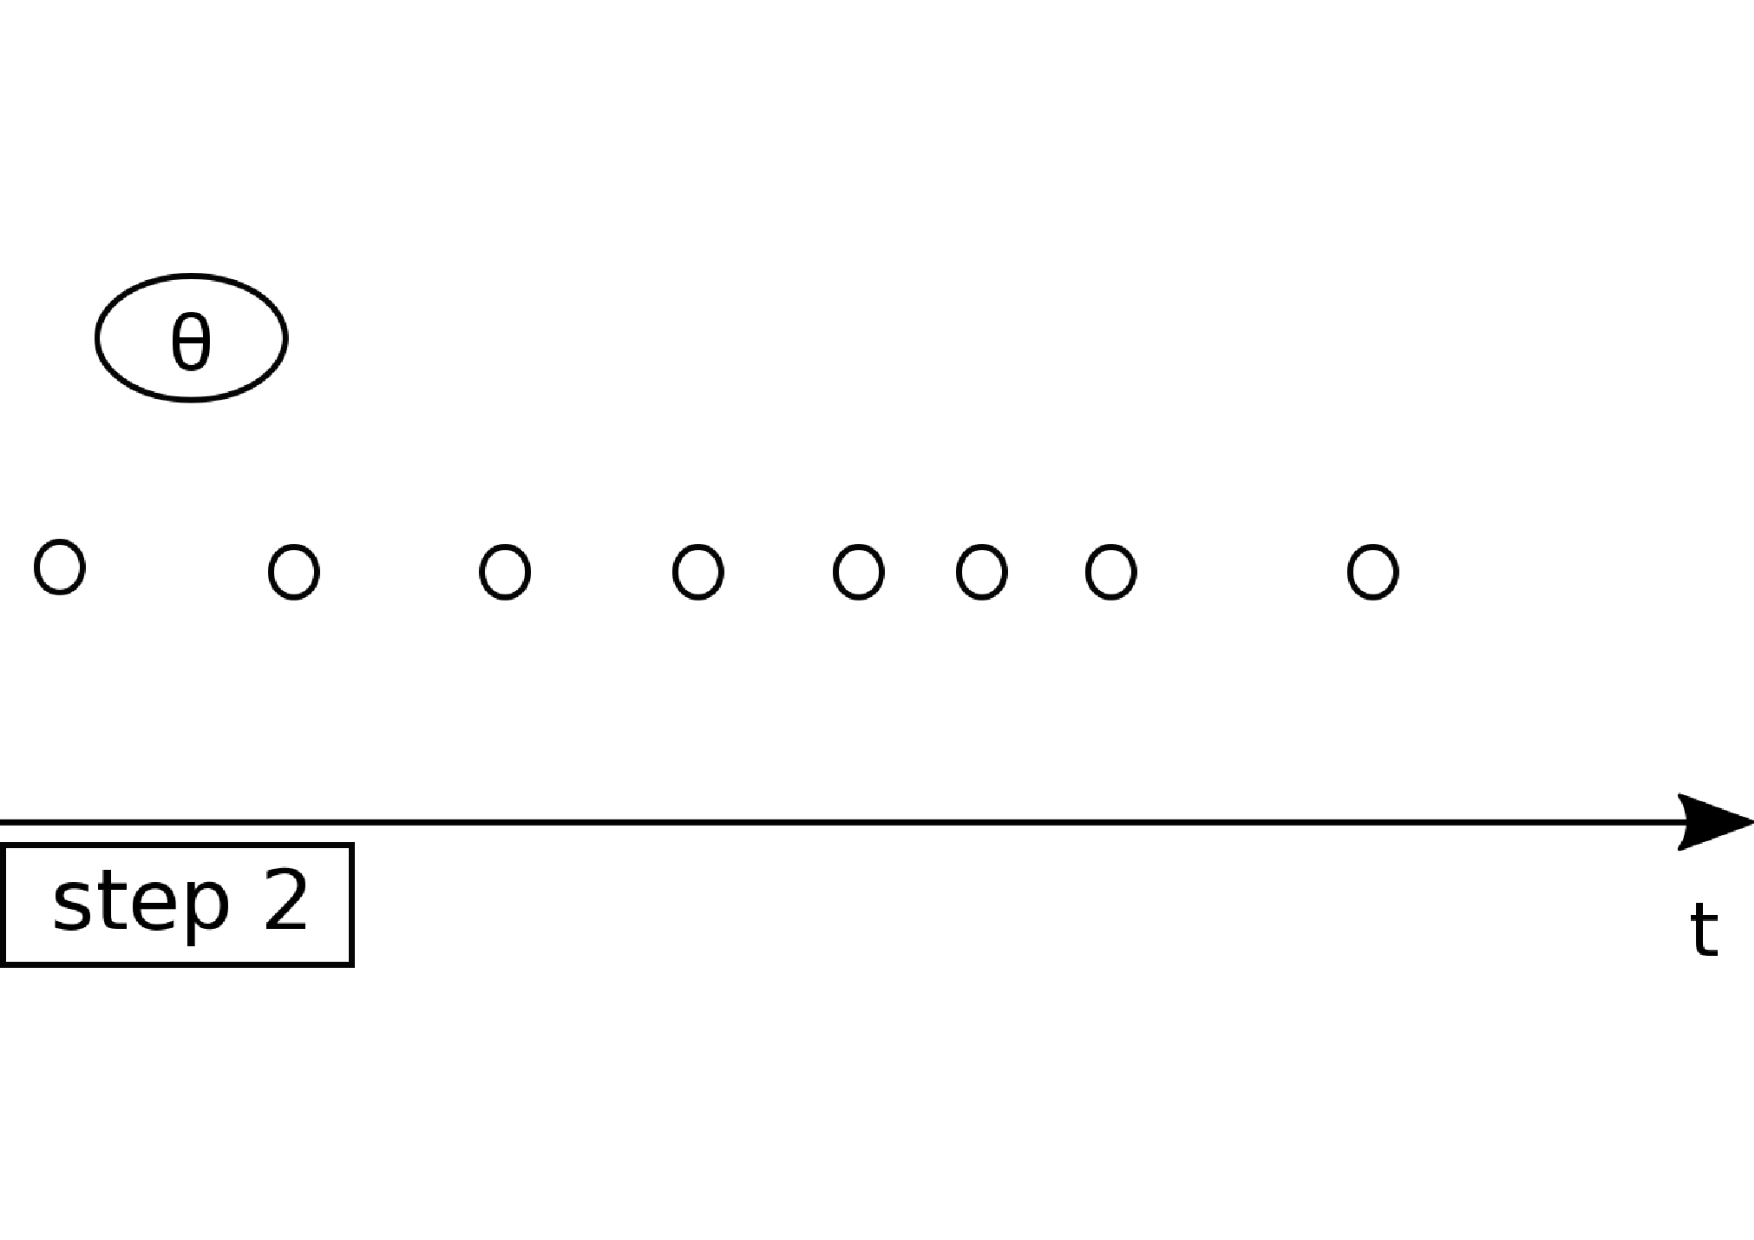
\includegraphics [width=0.70\textwidth, angle=0]{figs/plotn2.pdf}
    \vspace{-0 in}
  \end{minipage}
  \begin{minipage}[!hp]{0.45\linewidth}
  \centering
    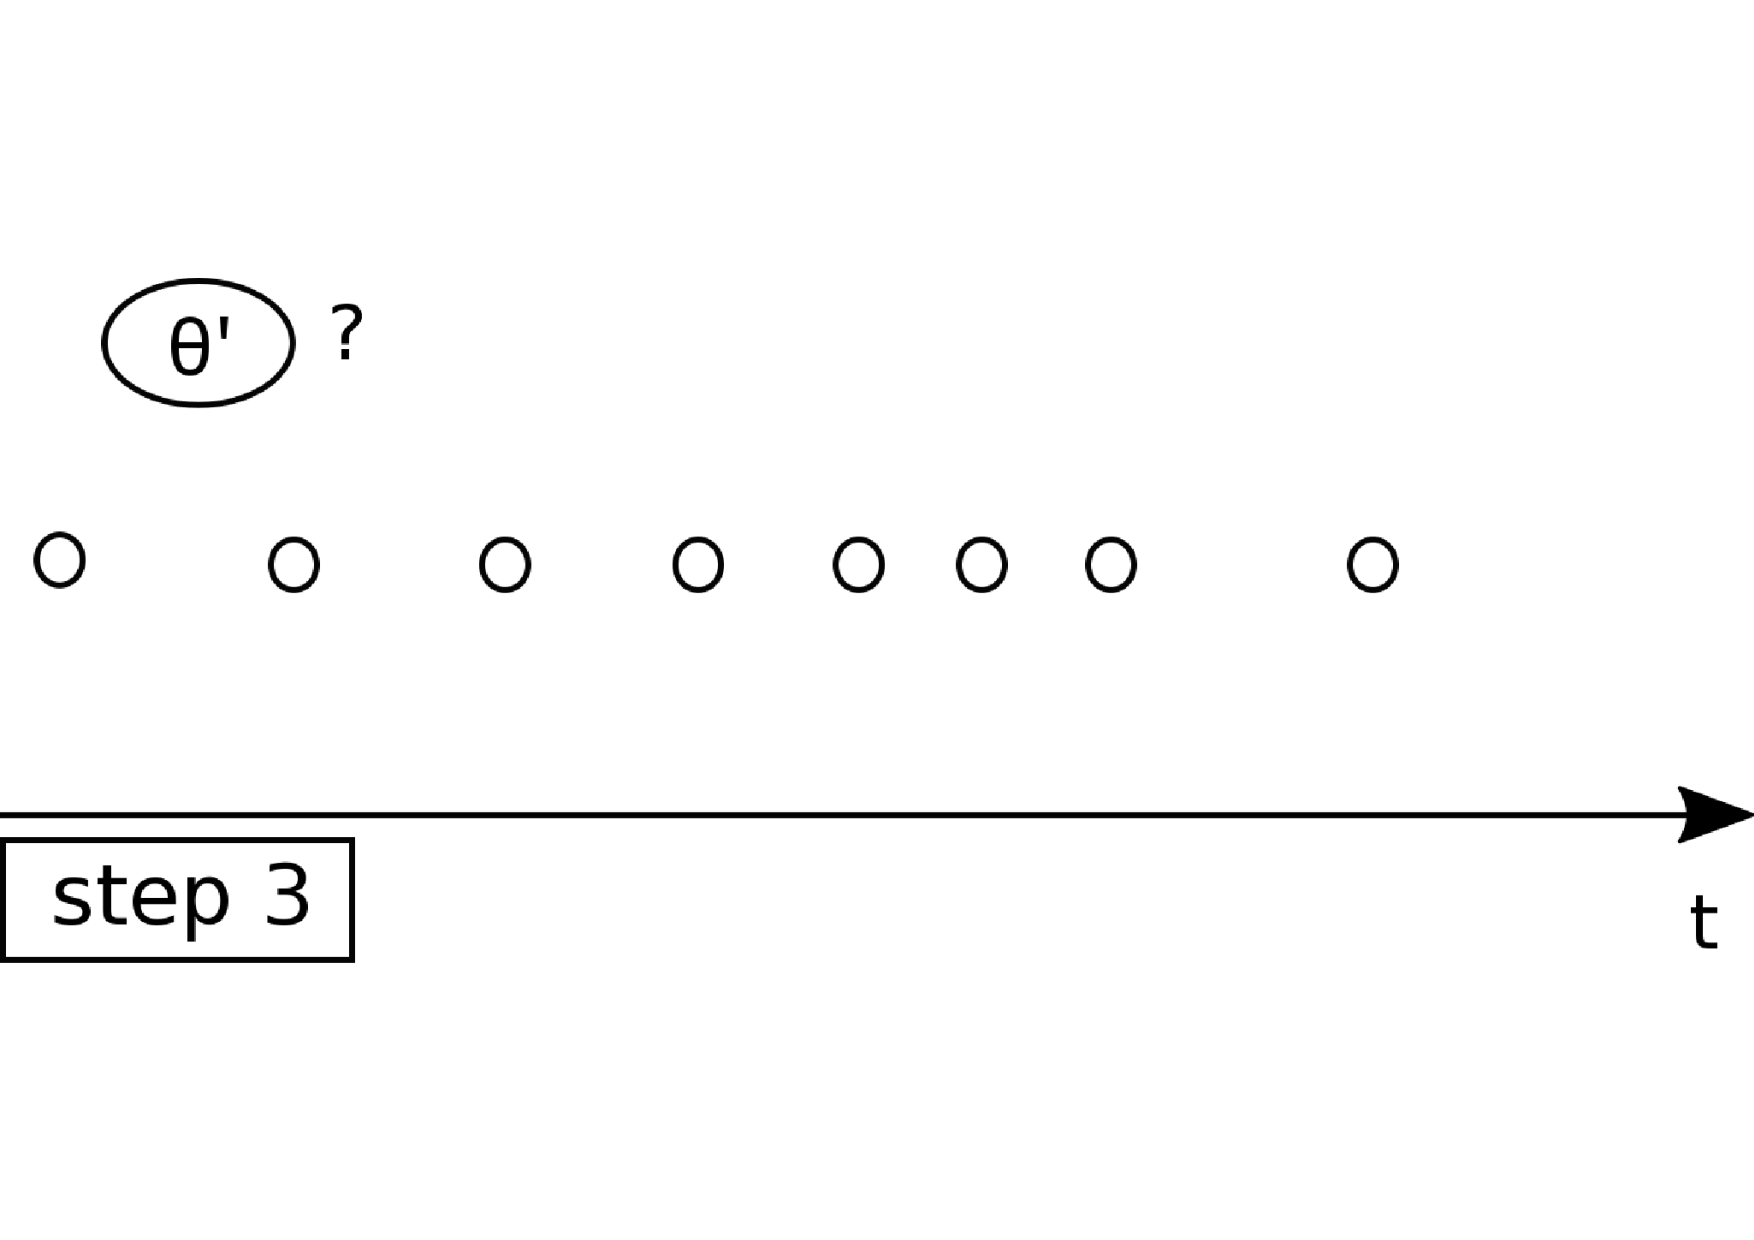
\includegraphics [width=0.70\textwidth, angle=0]{figs/plotn3.pdf}
    \vspace{-0 in}
  \end{minipage}
  \begin{minipage}[!hp]{0.45\linewidth}
  \centering
    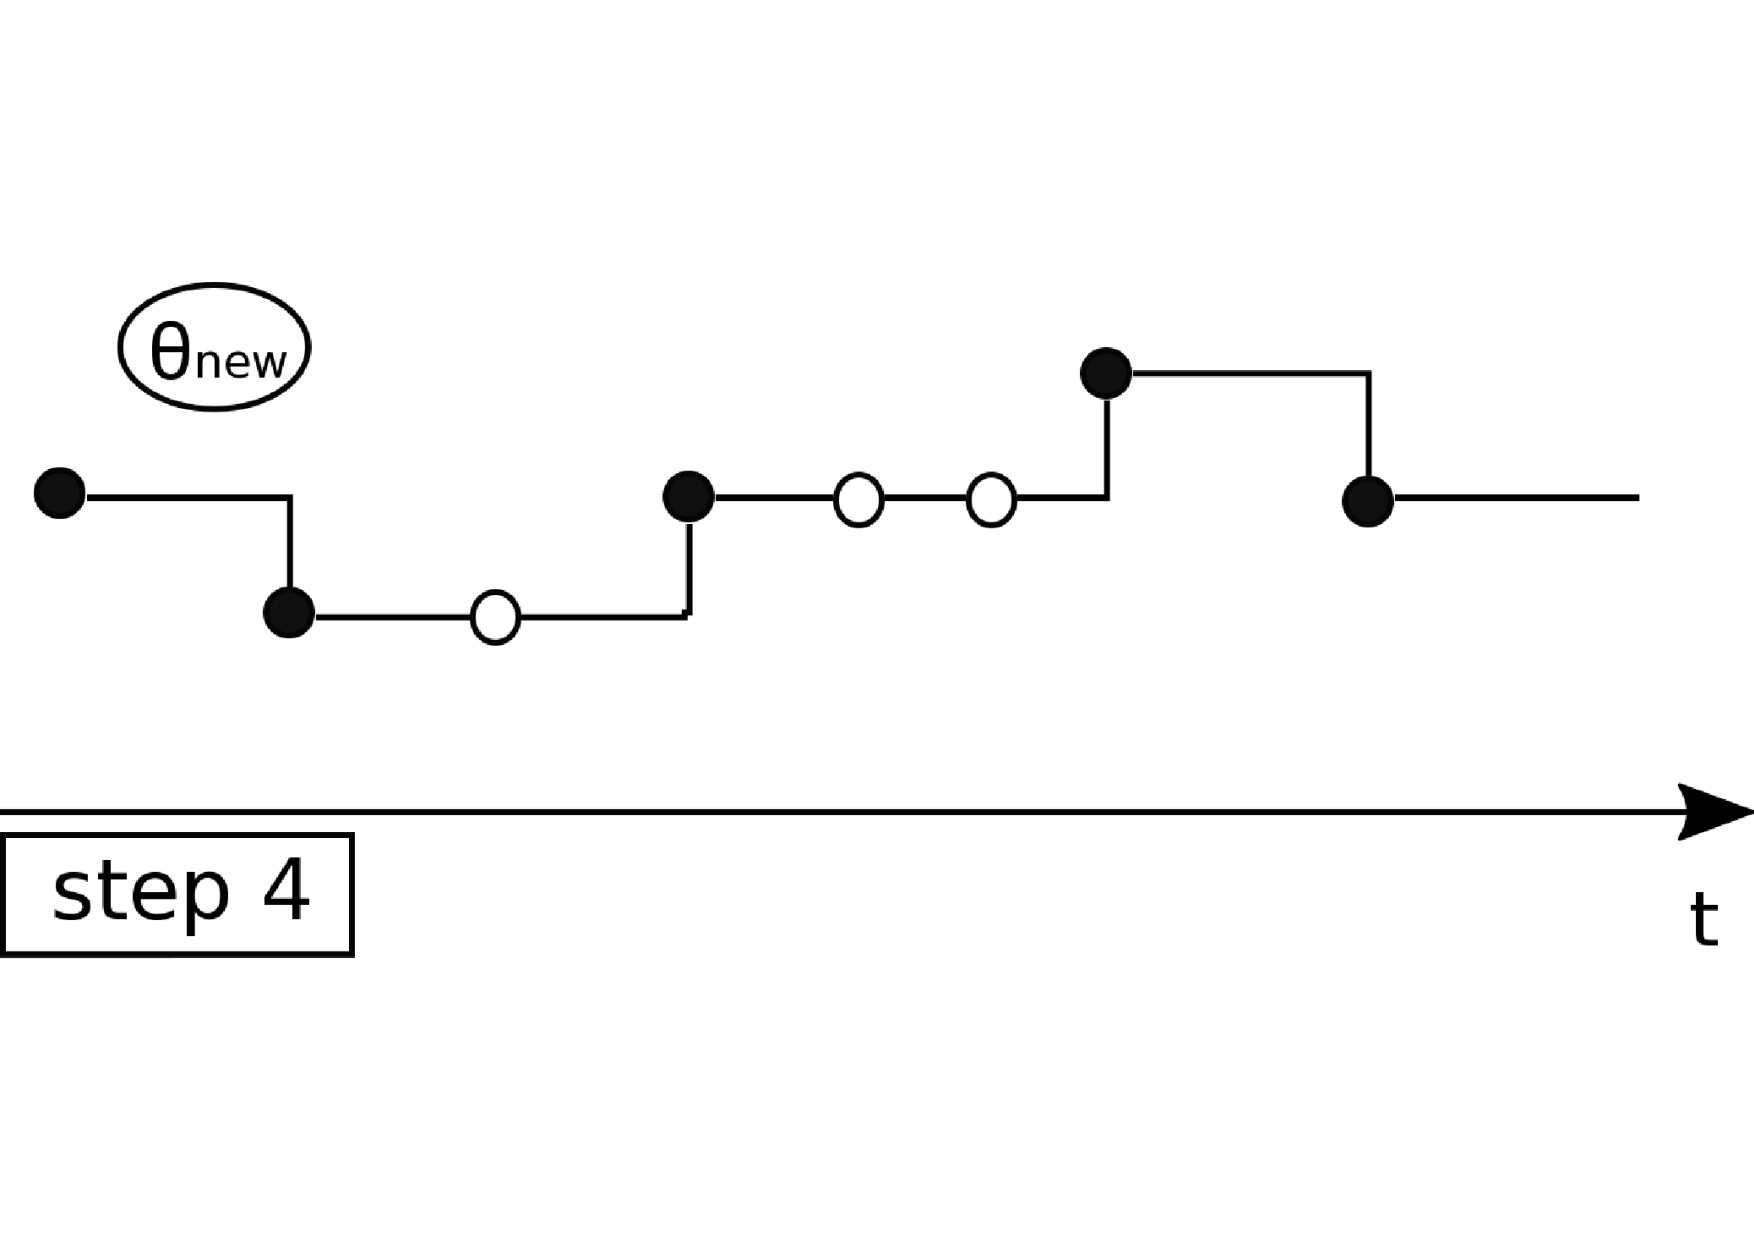
\includegraphics [width=0.70\textwidth, angle=0]{figs/plotn4.pdf}
    \vspace{-0 in}
  \end{minipage}
  \begin{minipage}[!hp]{0.45\linewidth}
  \centering
    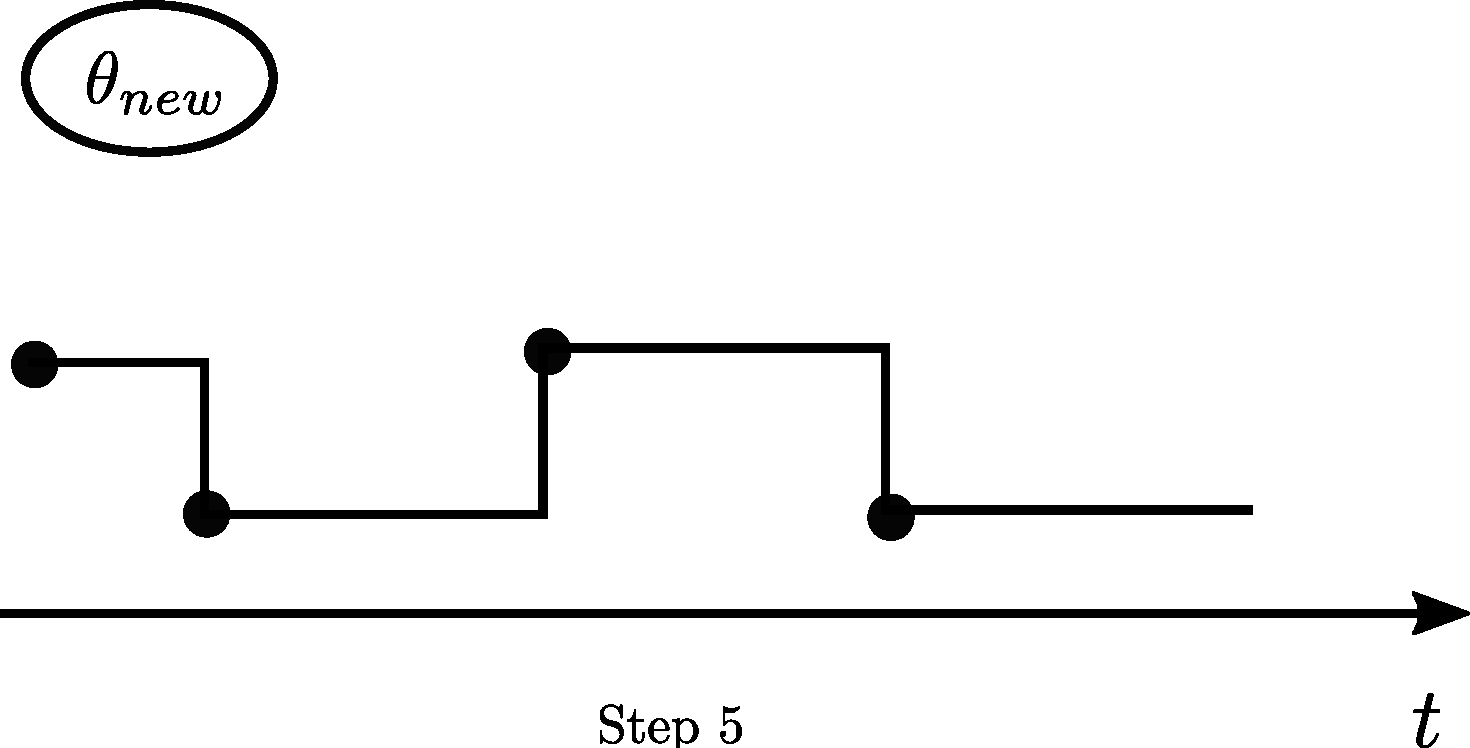
\includegraphics [width=0.70\textwidth, angle=0]{figs/plotn5.pdf}
    \vspace{-0 in}
  \end{minipage}
  \caption{\Naive\ MH-algorithm: Step 0 to 2: sample thinned events
  and discard state information to get a random grid. Step 3: 
propose a new parameter $\theta'$, and accept or reject by making
a forward pass on the grid. Steps 4 to 5: make a backward pass using
the accepted parameter and discard self-transitions to produce a new
trajectory.}
   \label{fig:naive_mh}
  \end{figure}

\setlength{\unitlength}{0.8cm}
  \begin{figure}[h!]
  \centering
  \begin{minipage}[!hp]{0.45\linewidth}
  \centering
    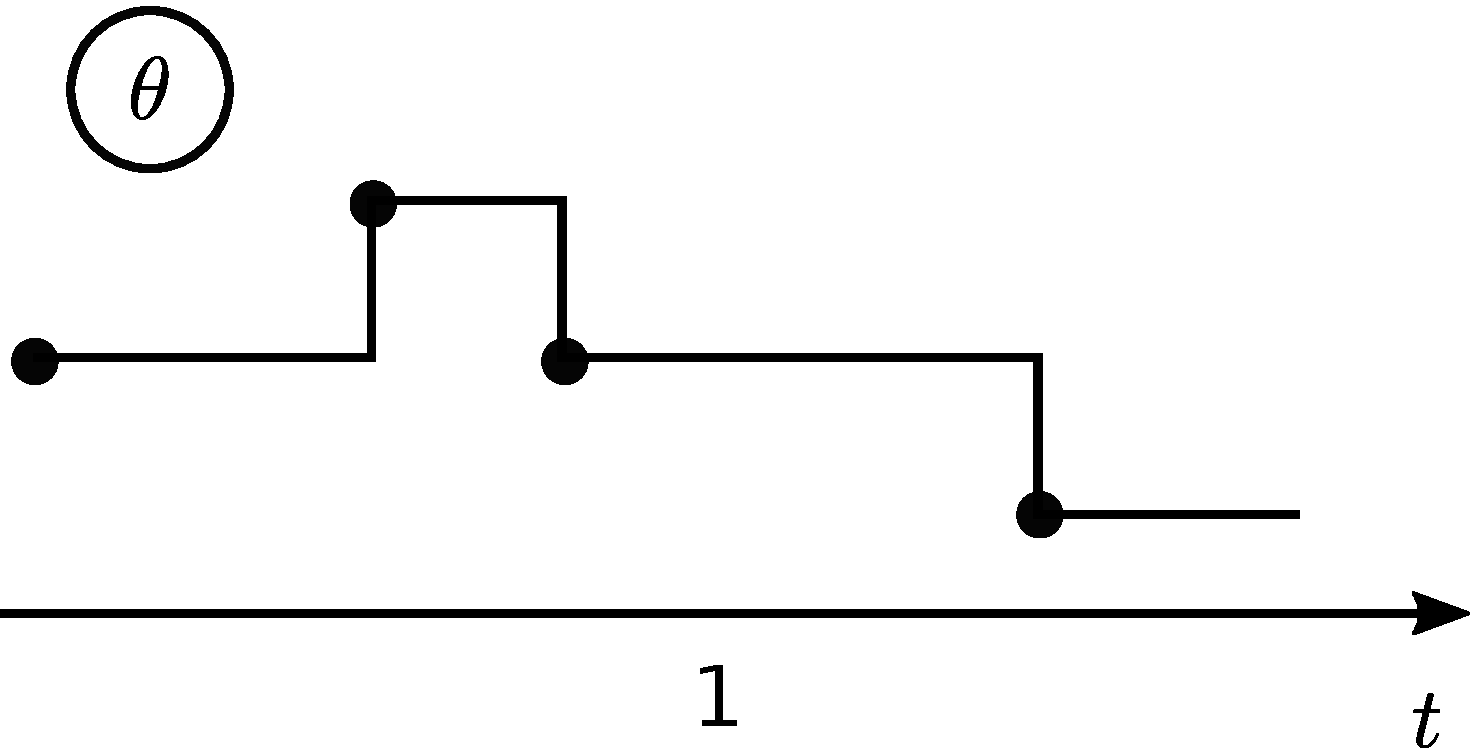
\includegraphics [width=0.70\textwidth, angle=0]{figs/plot0.pdf}
      \end{minipage}
  \begin{minipage}[hp]{0.45\linewidth}
  \centering
    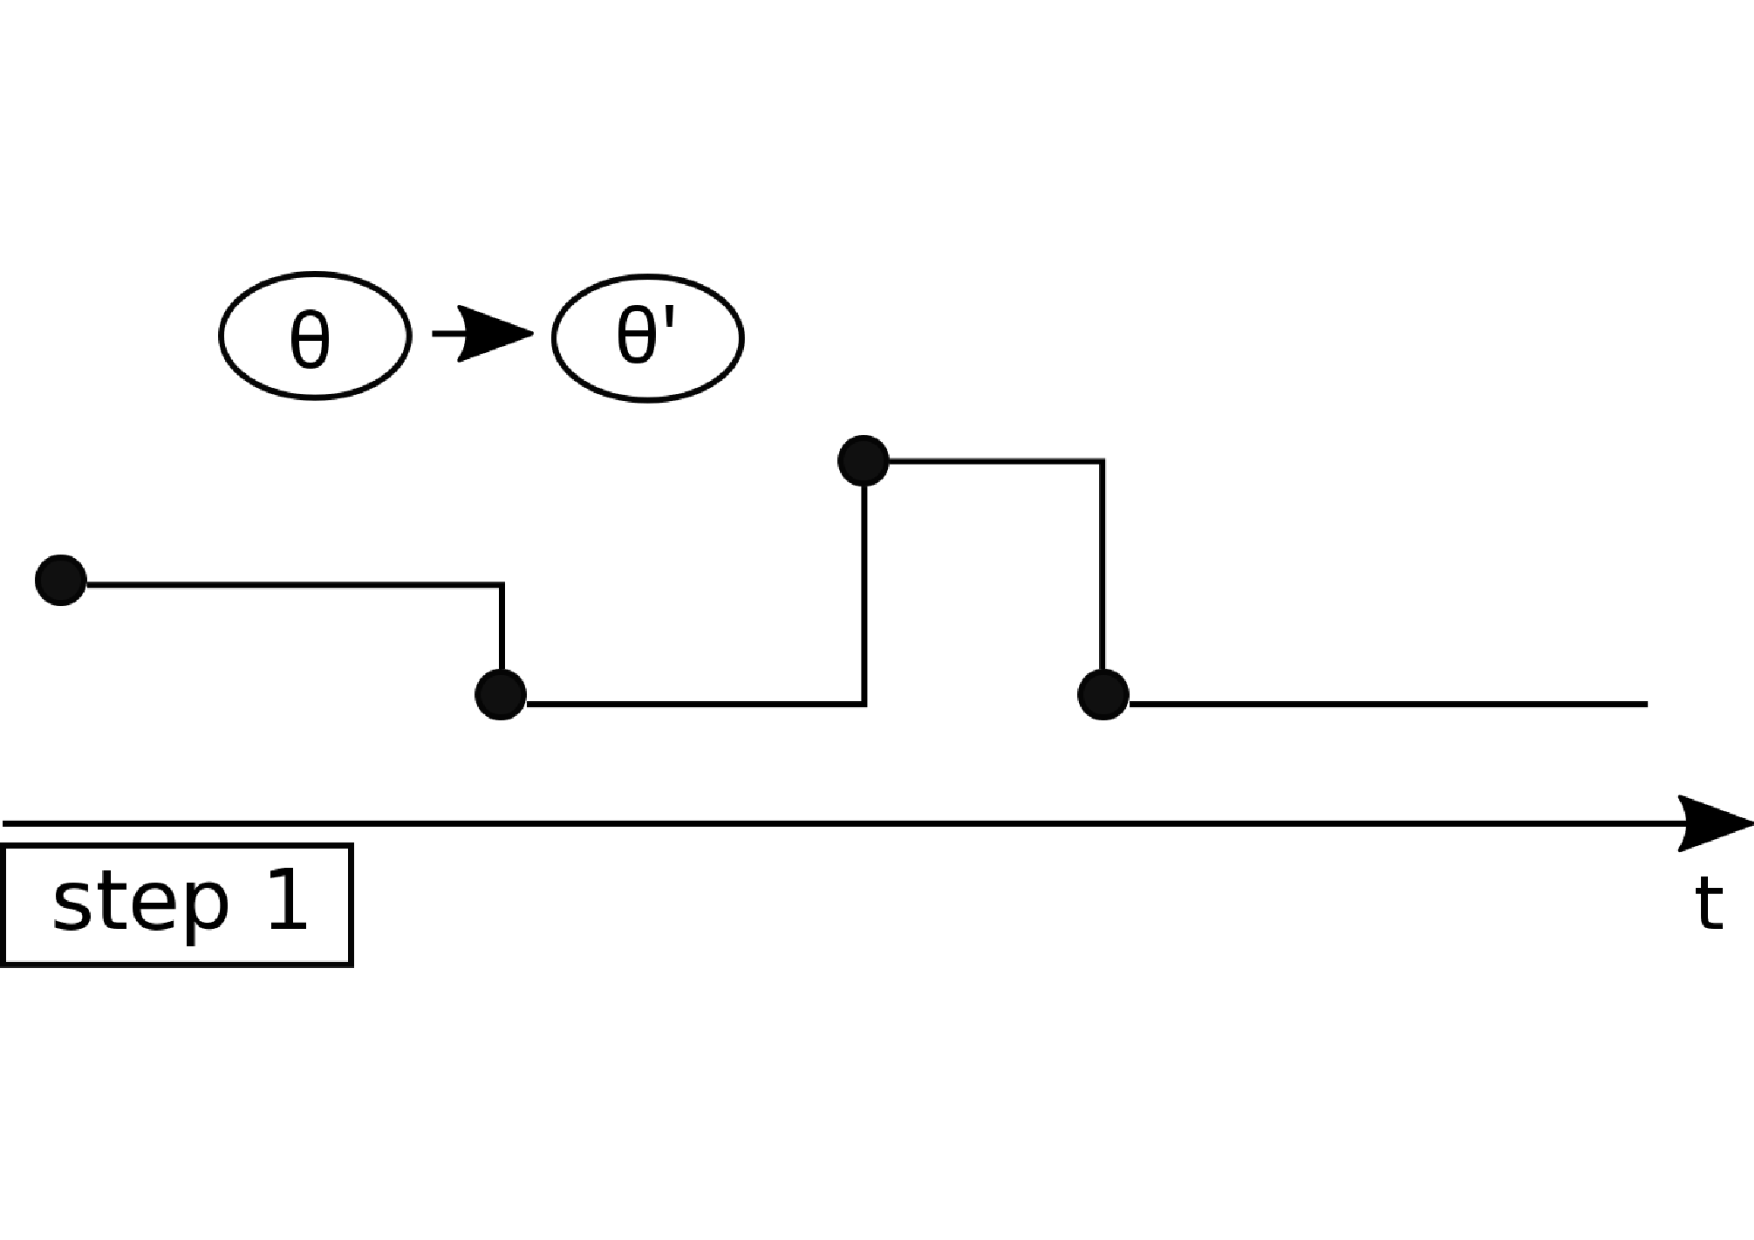
\includegraphics [width=0.70\textwidth, angle=0]{figs/plot1.pdf}
    \vspace{-0 in}
  \end{minipage}
  \begin{minipage}[hp]{0.45\linewidth}
  \centering
    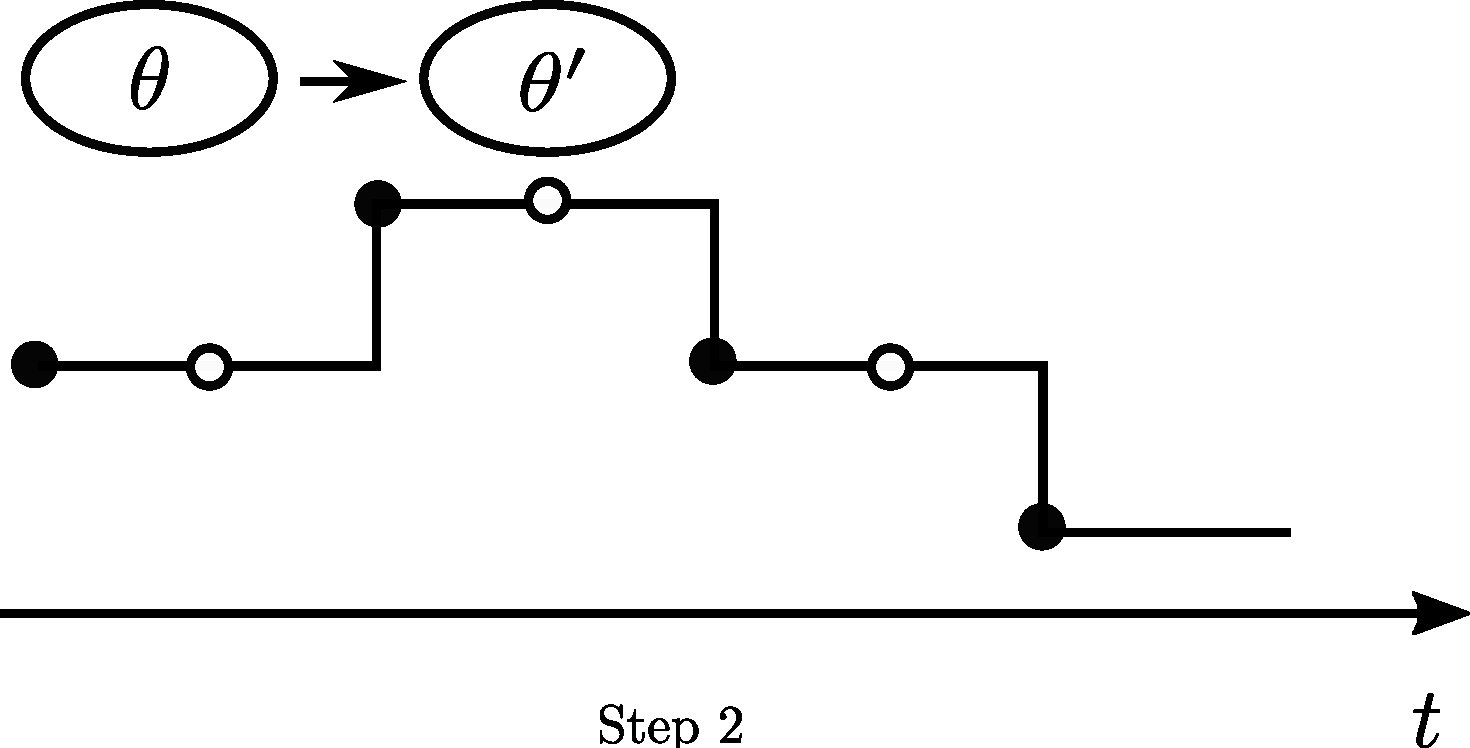
\includegraphics [width=0.70\textwidth, angle=0]{figs/plot2.pdf}
    \vspace{-0 in}
  \end{minipage}
  \begin{minipage}[hp]{0.45\linewidth}
  \centering
    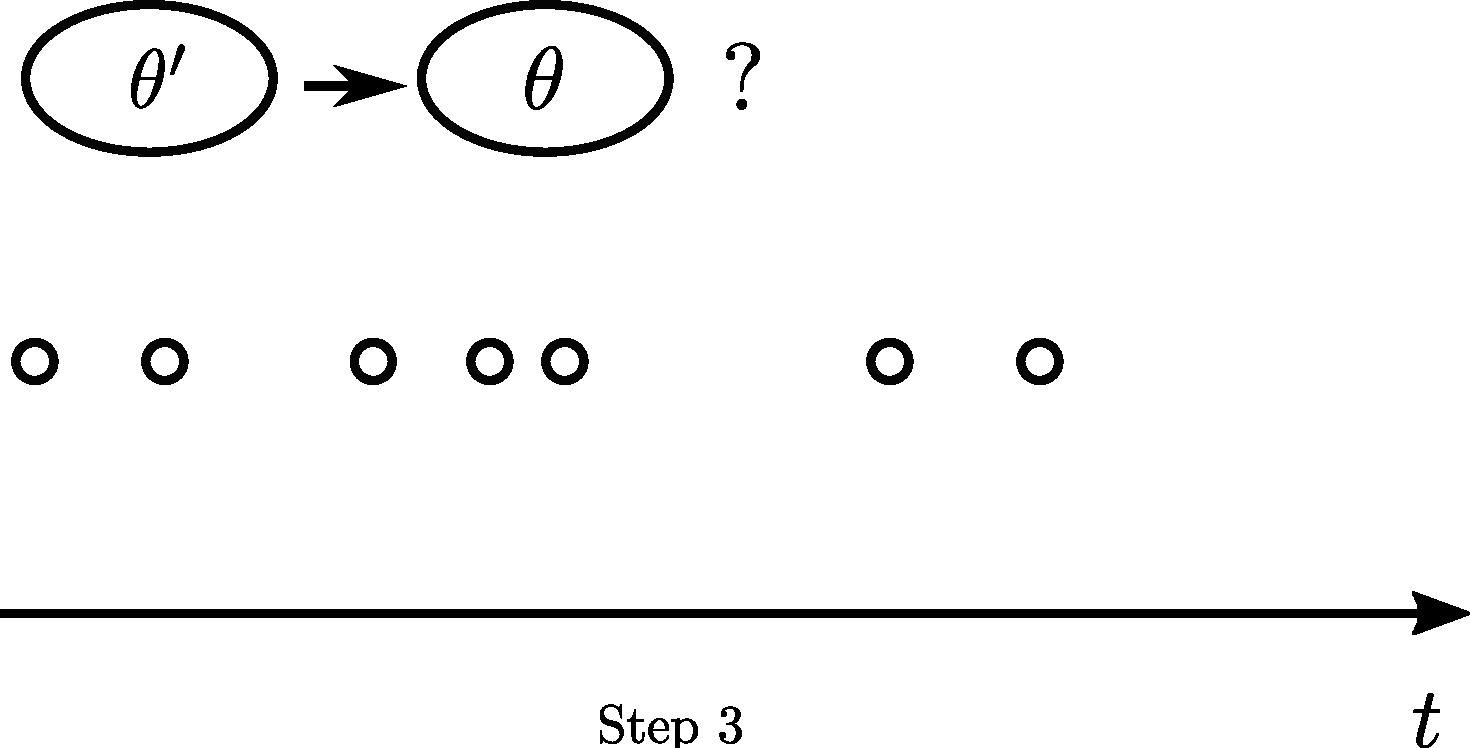
\includegraphics [width=0.70\textwidth, angle=0]{figs/plot3.pdf}
    \vspace{-0 in}
  \end{minipage}
% \begin{minipage}[hp]{0.45\linewidth}
% \centering
%   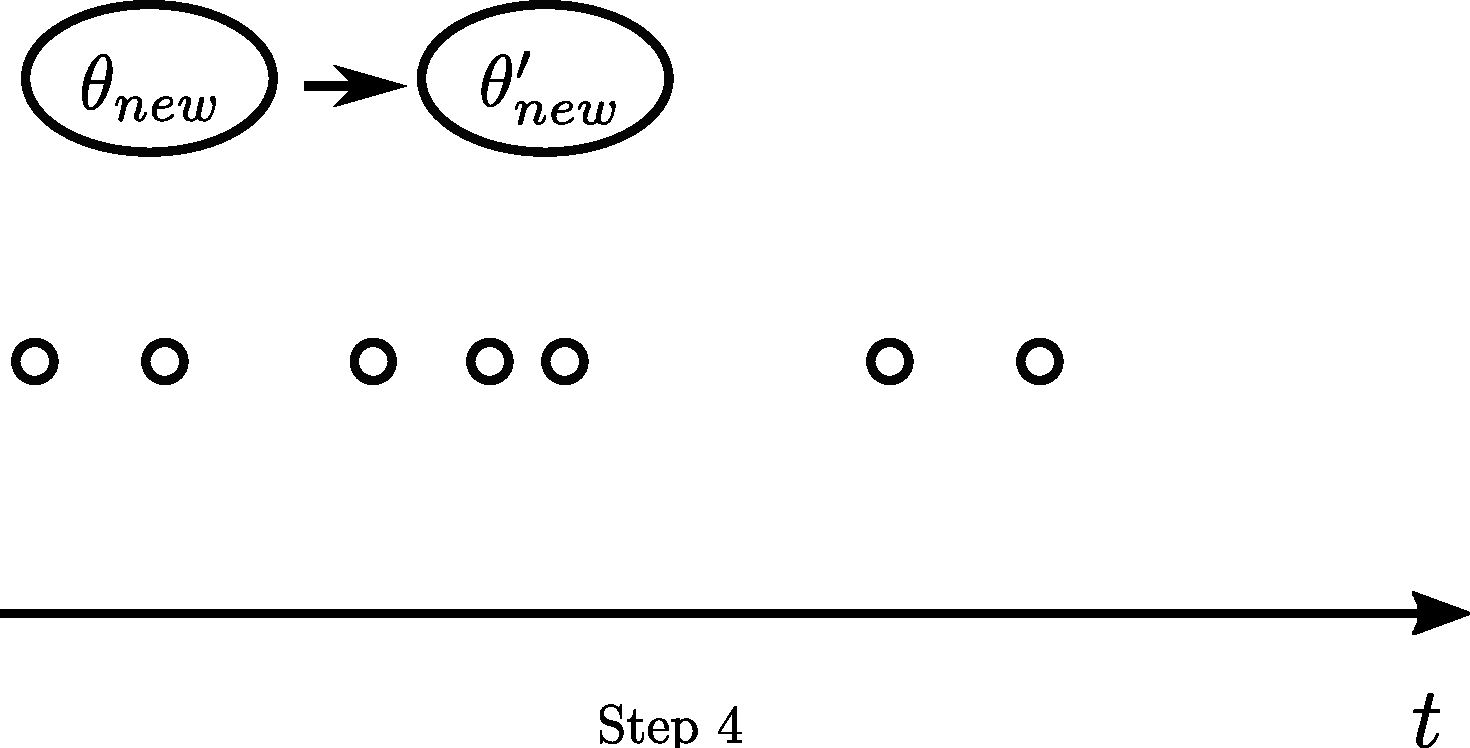
\includegraphics [width=0.70\textwidth, angle=0]{figs/plot4.pdf}
%   \vspace{-0 in}
% \end{minipage}
  \begin{minipage}[hp]{0.45\linewidth}
  \centering
    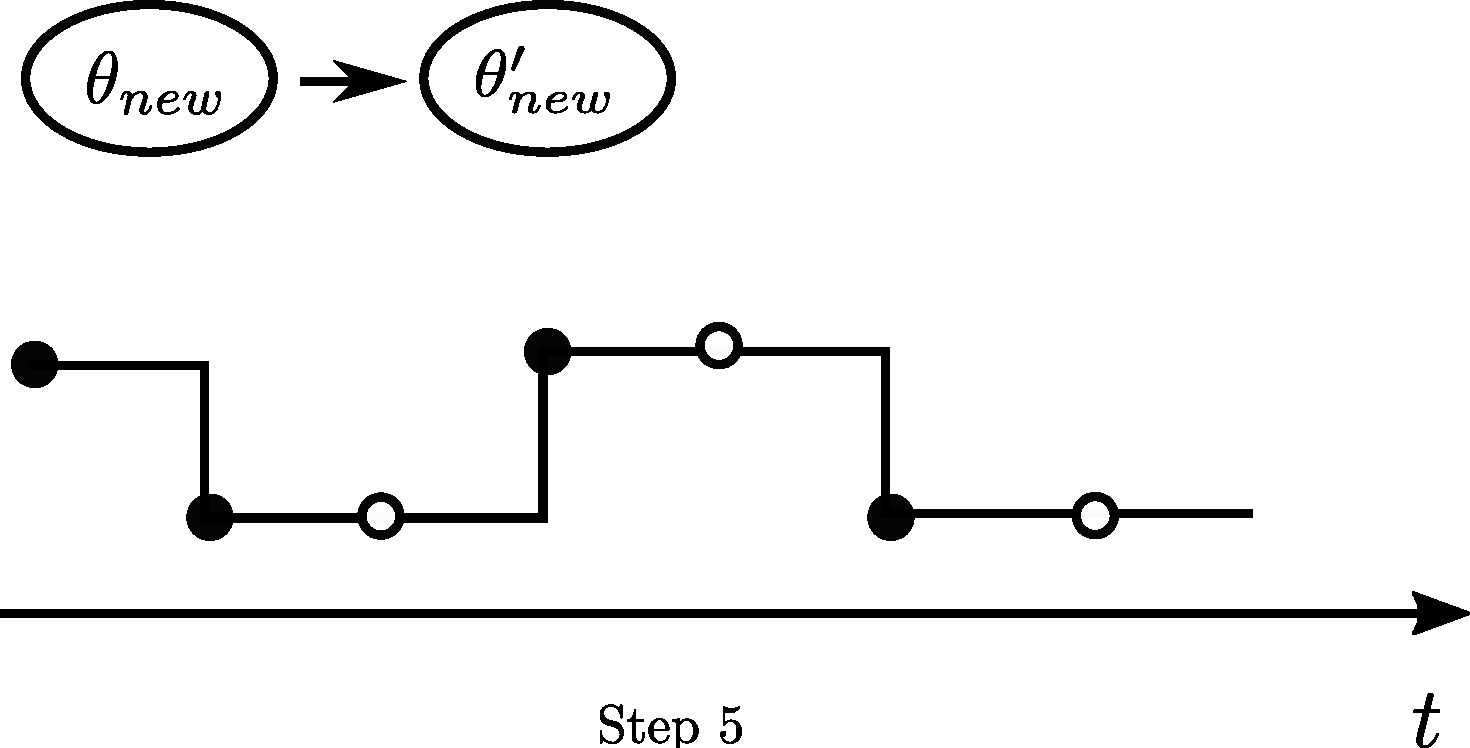
\includegraphics [width=0.70\textwidth, angle=0]{figs/plot5.pdf}
    \vspace{-0 in}
  \end{minipage}
  \begin{minipage}[hp]{0.45\linewidth}
  \centering
    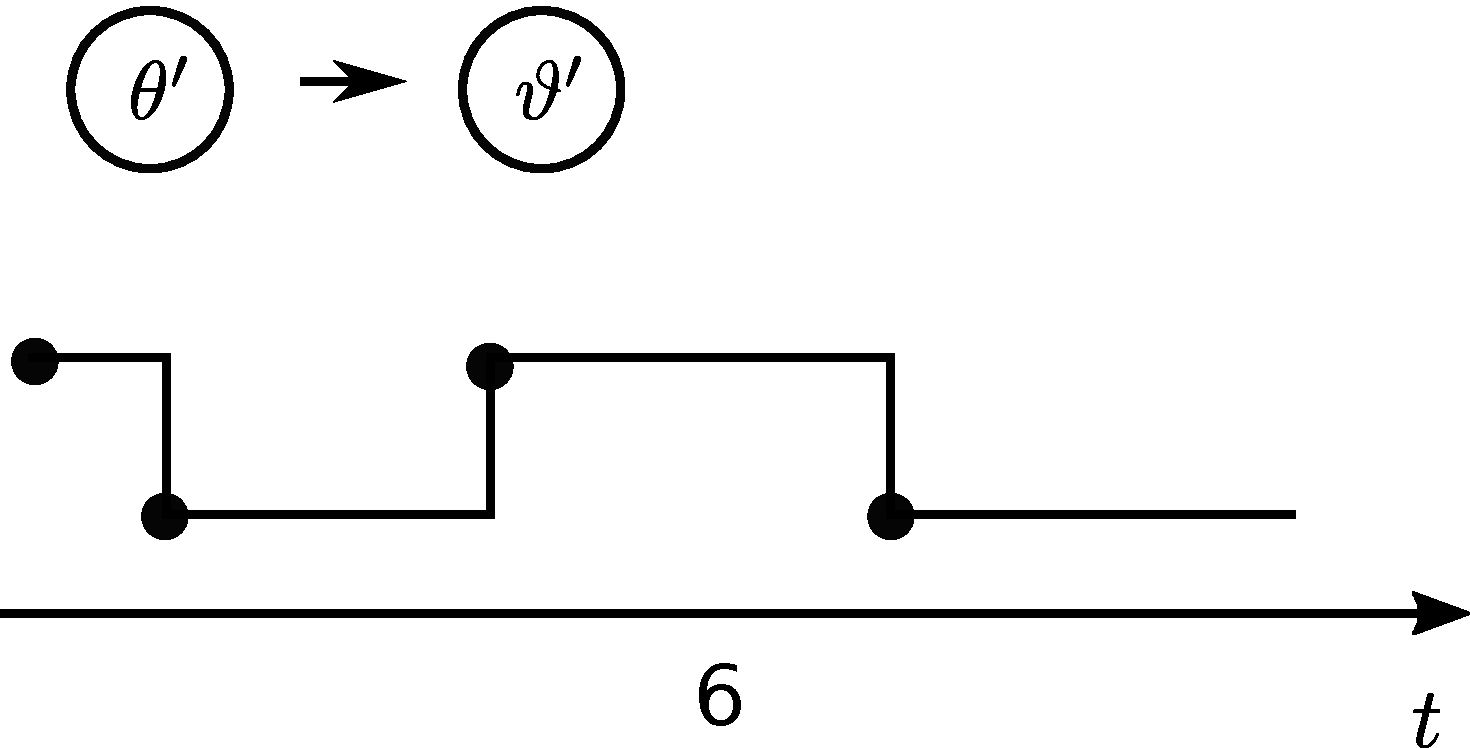
\includegraphics [width=0.70\textwidth, angle=0]{figs/plot6.pdf}
  \end{minipage}
    \caption{Improved MH algorithm: Steps 0-3: Starting with a trajectory and parameter $\theta$,
      simulate an auxiliary parameter $\theta^*$, and then the thinned events
      $U$ from a rate $\Omega(\theta) + \Omega(\theta^*) - A_{S(t)}$ Poisson
      process. Step 4: Propose swapping $\theta$ and $\theta^*$. Step 5:
      Run a forward pass to accept or reject this proposal, and use the accepted
    parameter to simulate a new trajectory. Step 6: Discard the thinned events.} 
   \label{fig:MH_improved}
  \end{figure}

\subsection{Additional results}
\vspace{-.4in}
  \begin{figure}[H]
  \centering
  \begin{minipage}[h!]{0.65\linewidth}
  \centering
    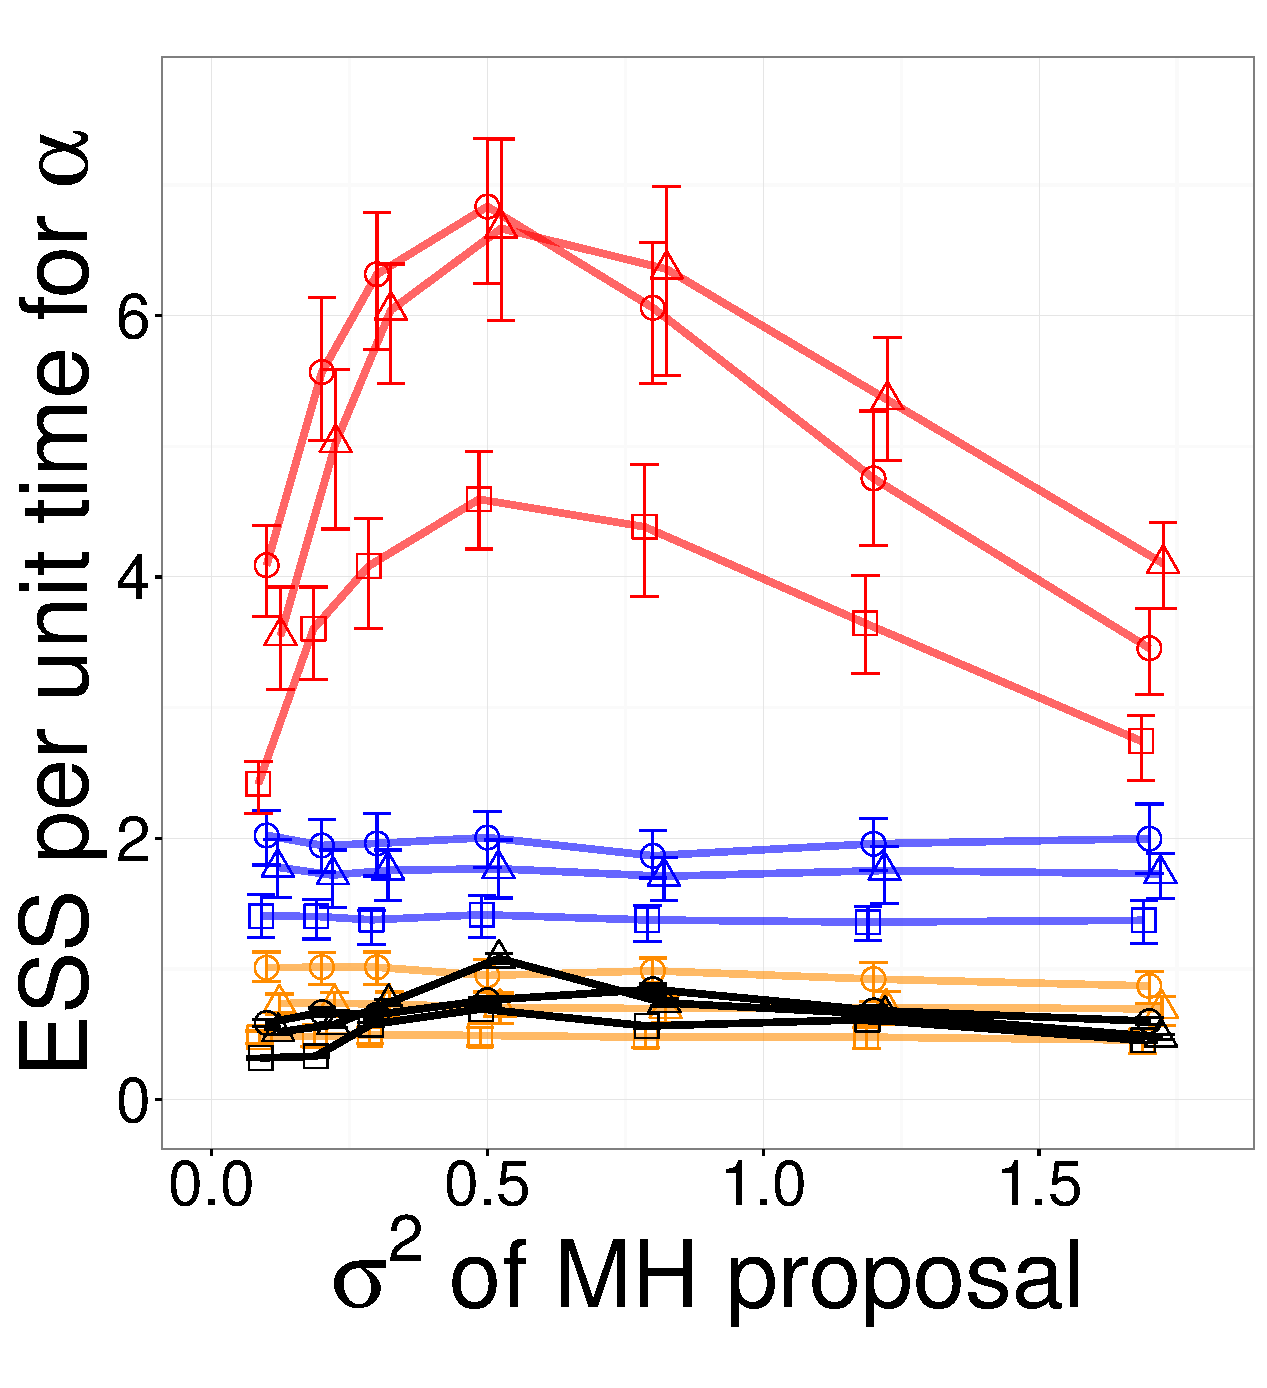
\includegraphics [width=0.44\textwidth, angle=0]{figs/exp_5_alpha.pdf}
    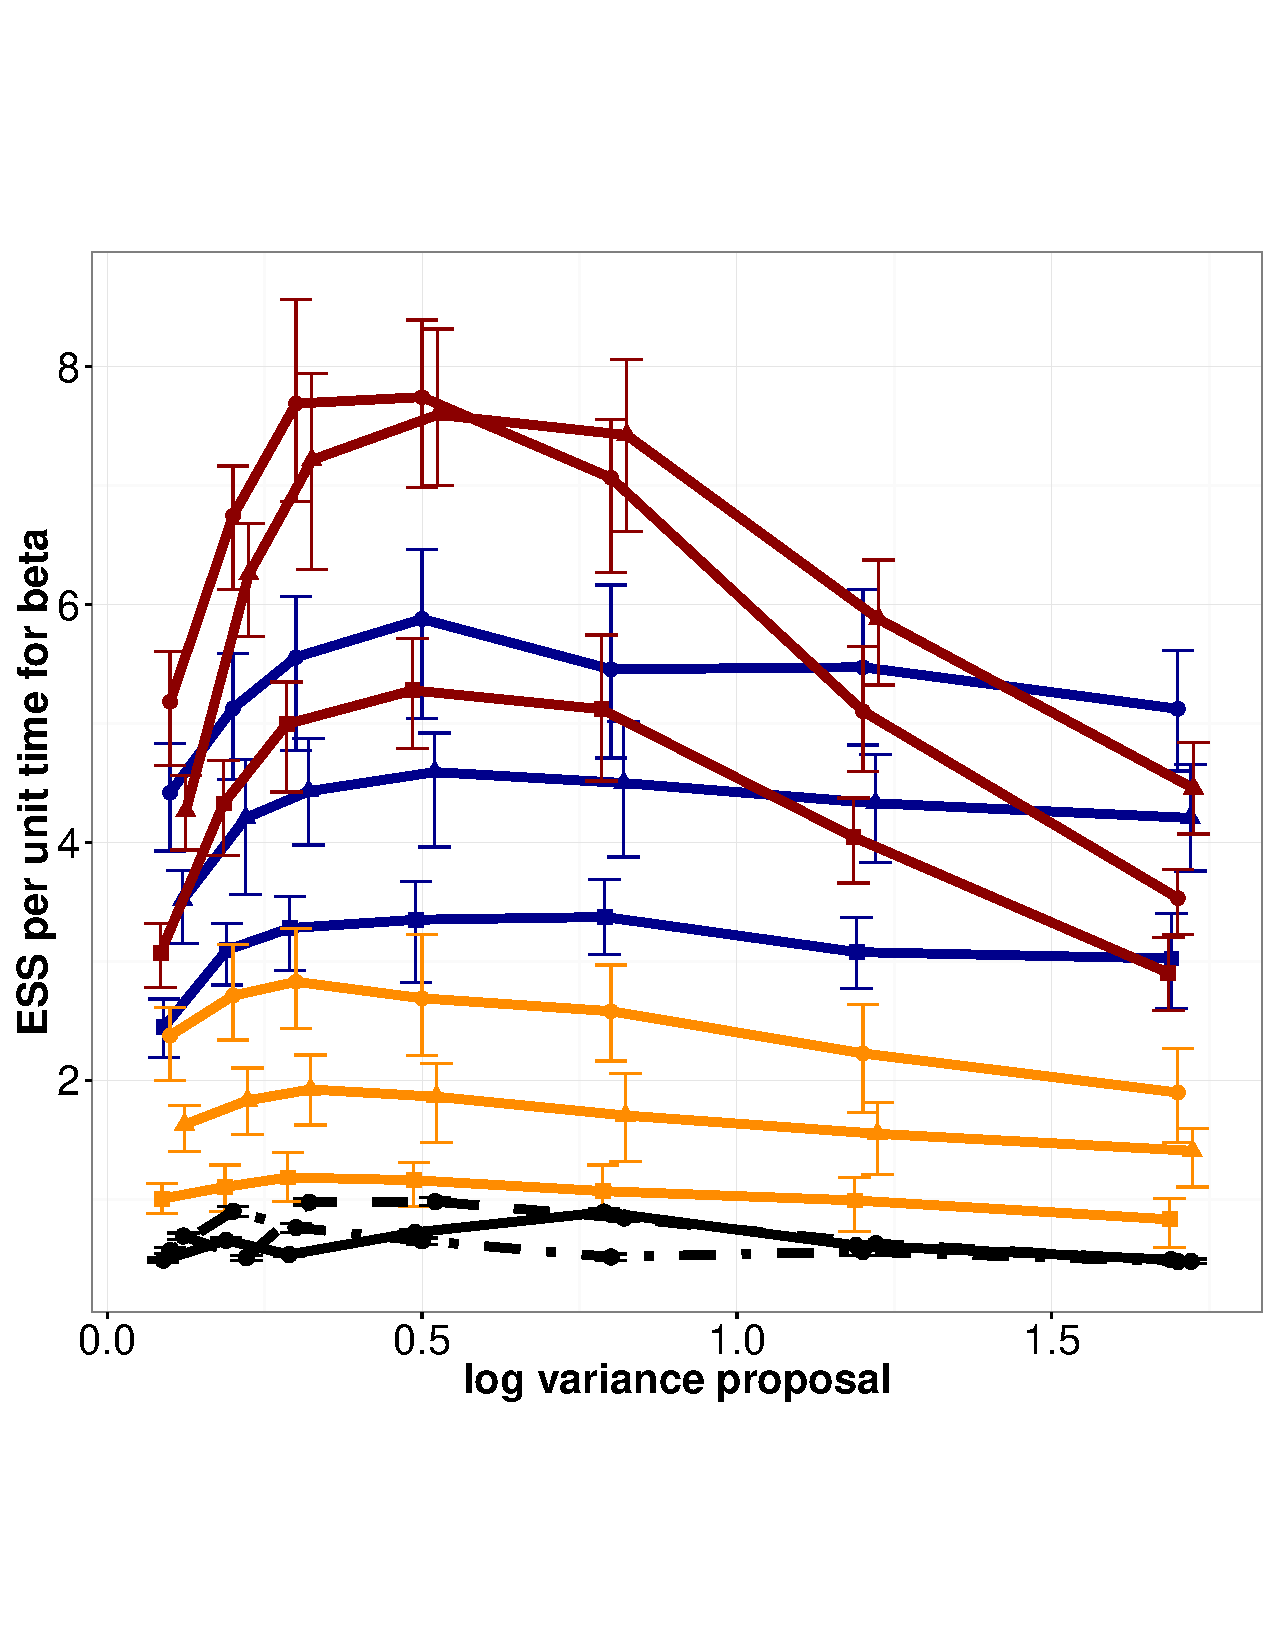
\includegraphics [width=0.44\textwidth, angle=0]{figs/exp_5_beta.pdf}
  \end{minipage}
  \begin{minipage}[!hp]{0.33\linewidth}
    \caption{ESS/sec for the synthetic  model, dimension 5. (Left, right) 
      are $(\alpha, \beta)$. Red, yellow, blue and black are the symmetrized MH,
  \naive\ MH, Gibbs and particle MCMC algorithm. Different symbols are
different settings of the algorithms, see section~\ref{sec:expts}.}
     \label{fig:ESS_EXP_D5}
  \end{minipage}
  \end{figure}
  %\centering

  \begin{figure}[H]
  \begin{minipage}[hp]{0.65\linewidth}
  \centering
    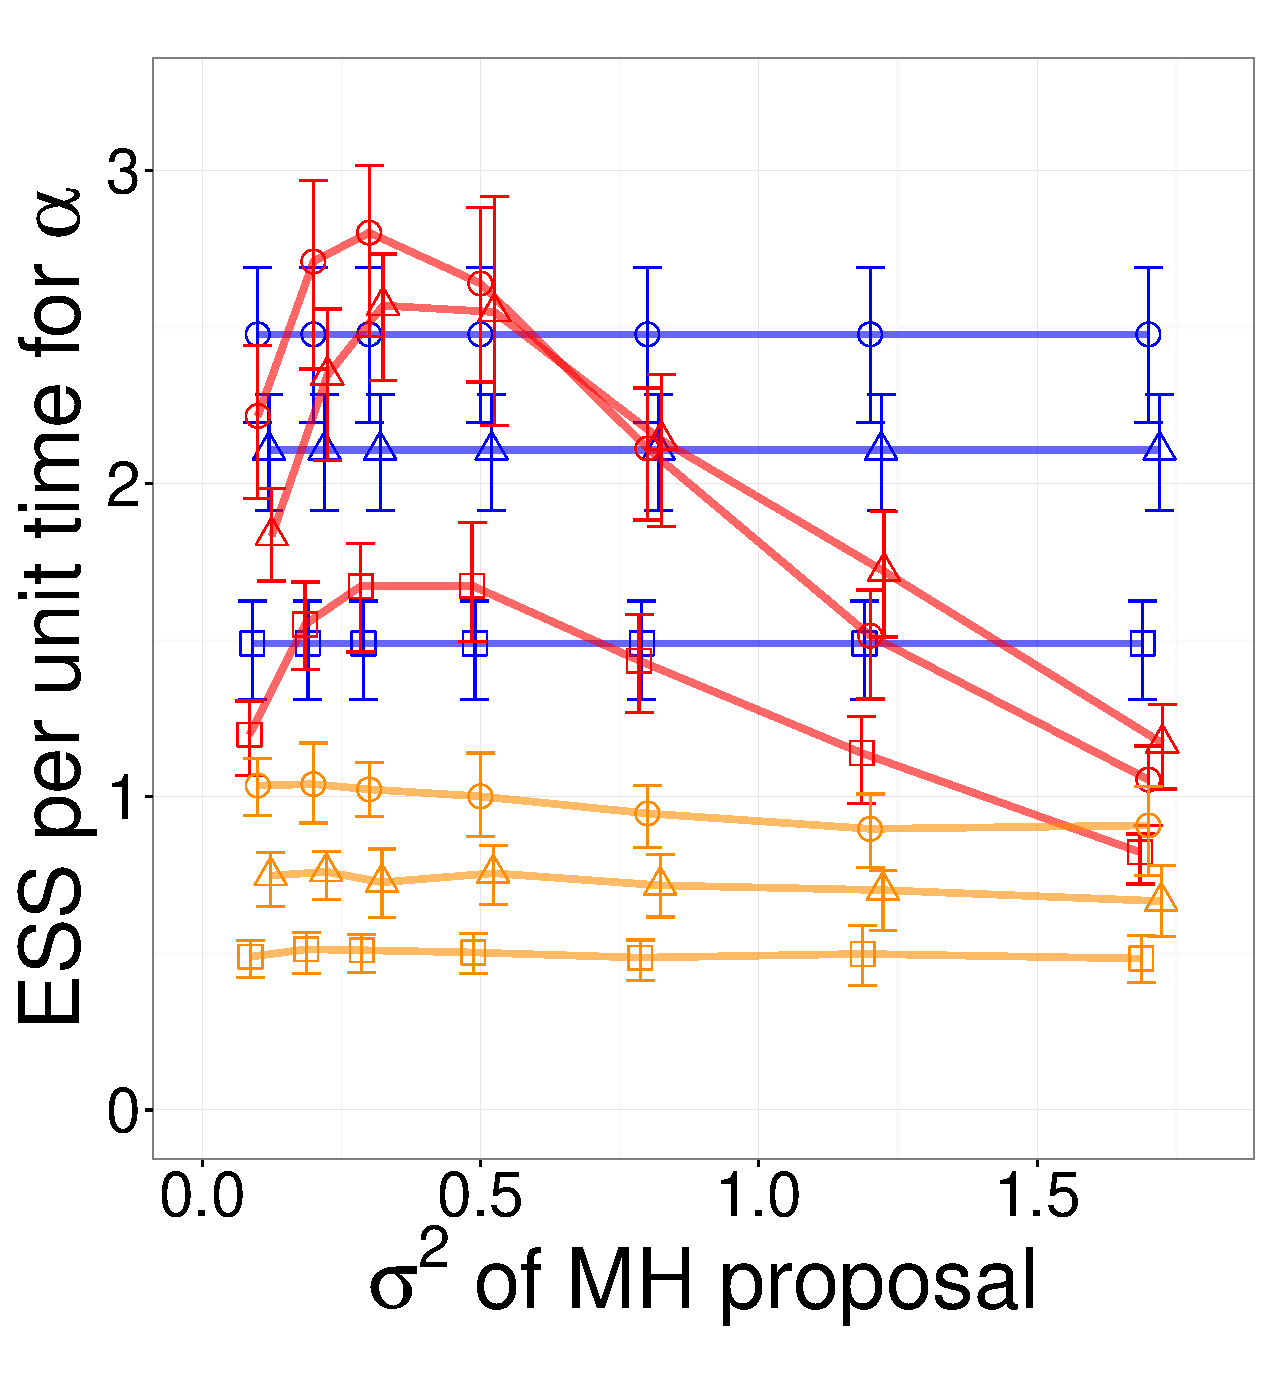
\includegraphics [width=0.44\textwidth, angle=0]{figs/q_5_alpha.pdf}
    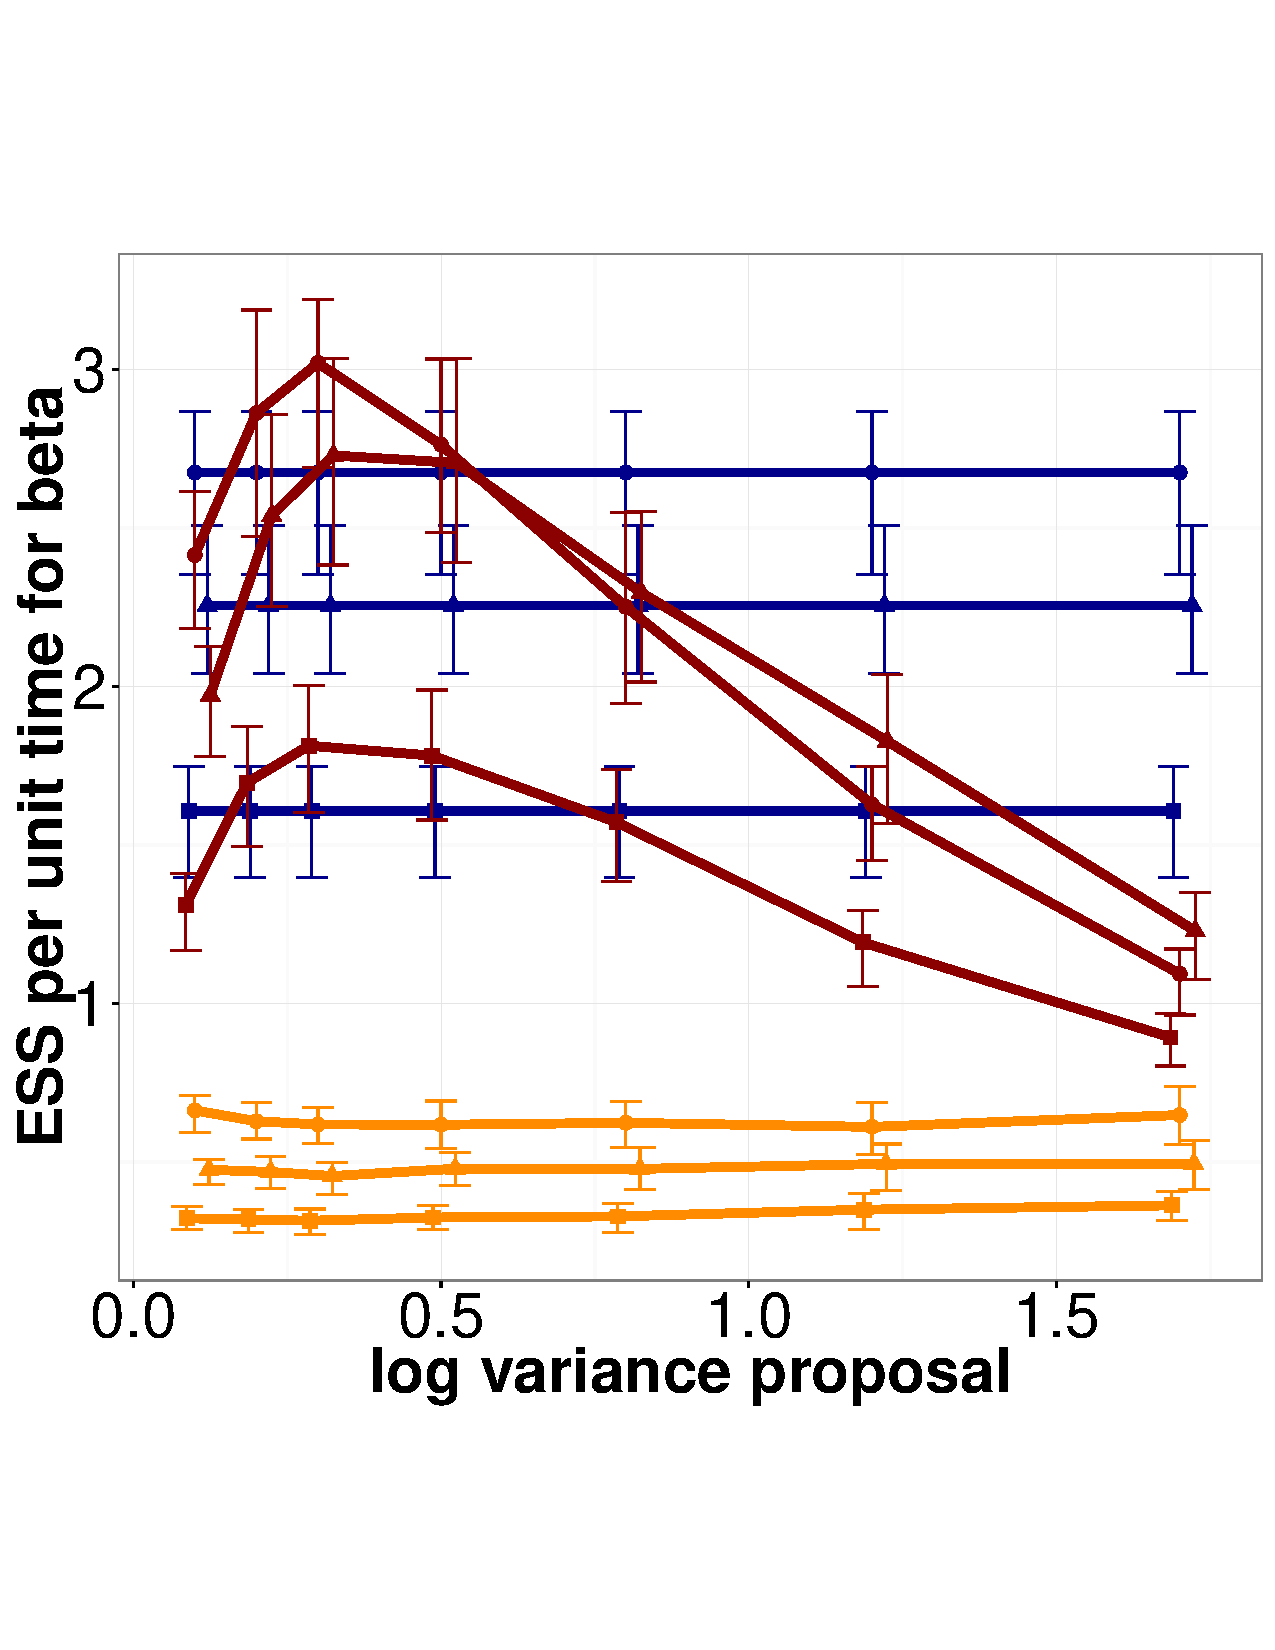
\includegraphics [width=0.44\textwidth, angle=0]{figs/q_5_beta.pdf}
  \end{minipage}
  \begin{minipage}[!hp]{0.33\linewidth}
    \caption{ESS/sec for the immigration model, with dimension 5. (Left, 
      right) are $(\alpha, \beta)$. Red, yellow, and blue curves are the symmetrized MH,
  \naive\ MH, Gibbs sampling and particle MCMC.}
     \label{fig:ESS_Q_D5}
  \end{minipage}
  \centering
  \begin{minipage}[!hp]{0.65\linewidth}
  \centering
    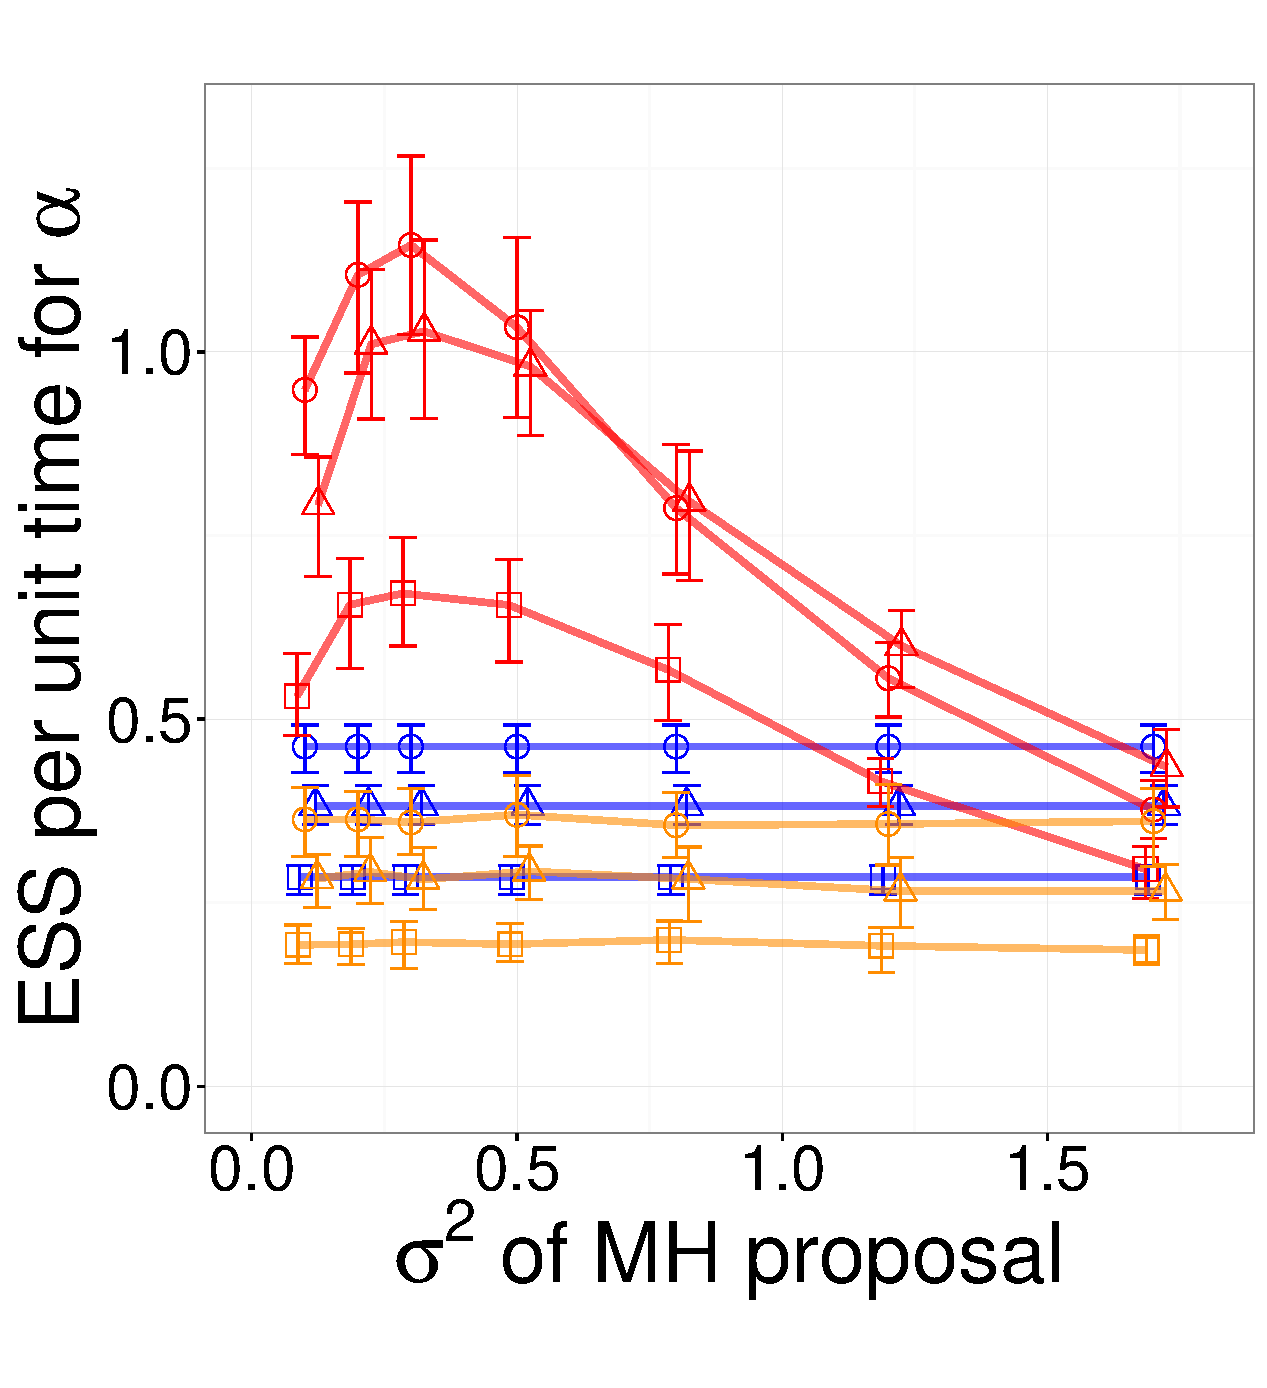
\includegraphics [width=0.44\textwidth, angle=0]{figs/pc_5_alpha.pdf}
    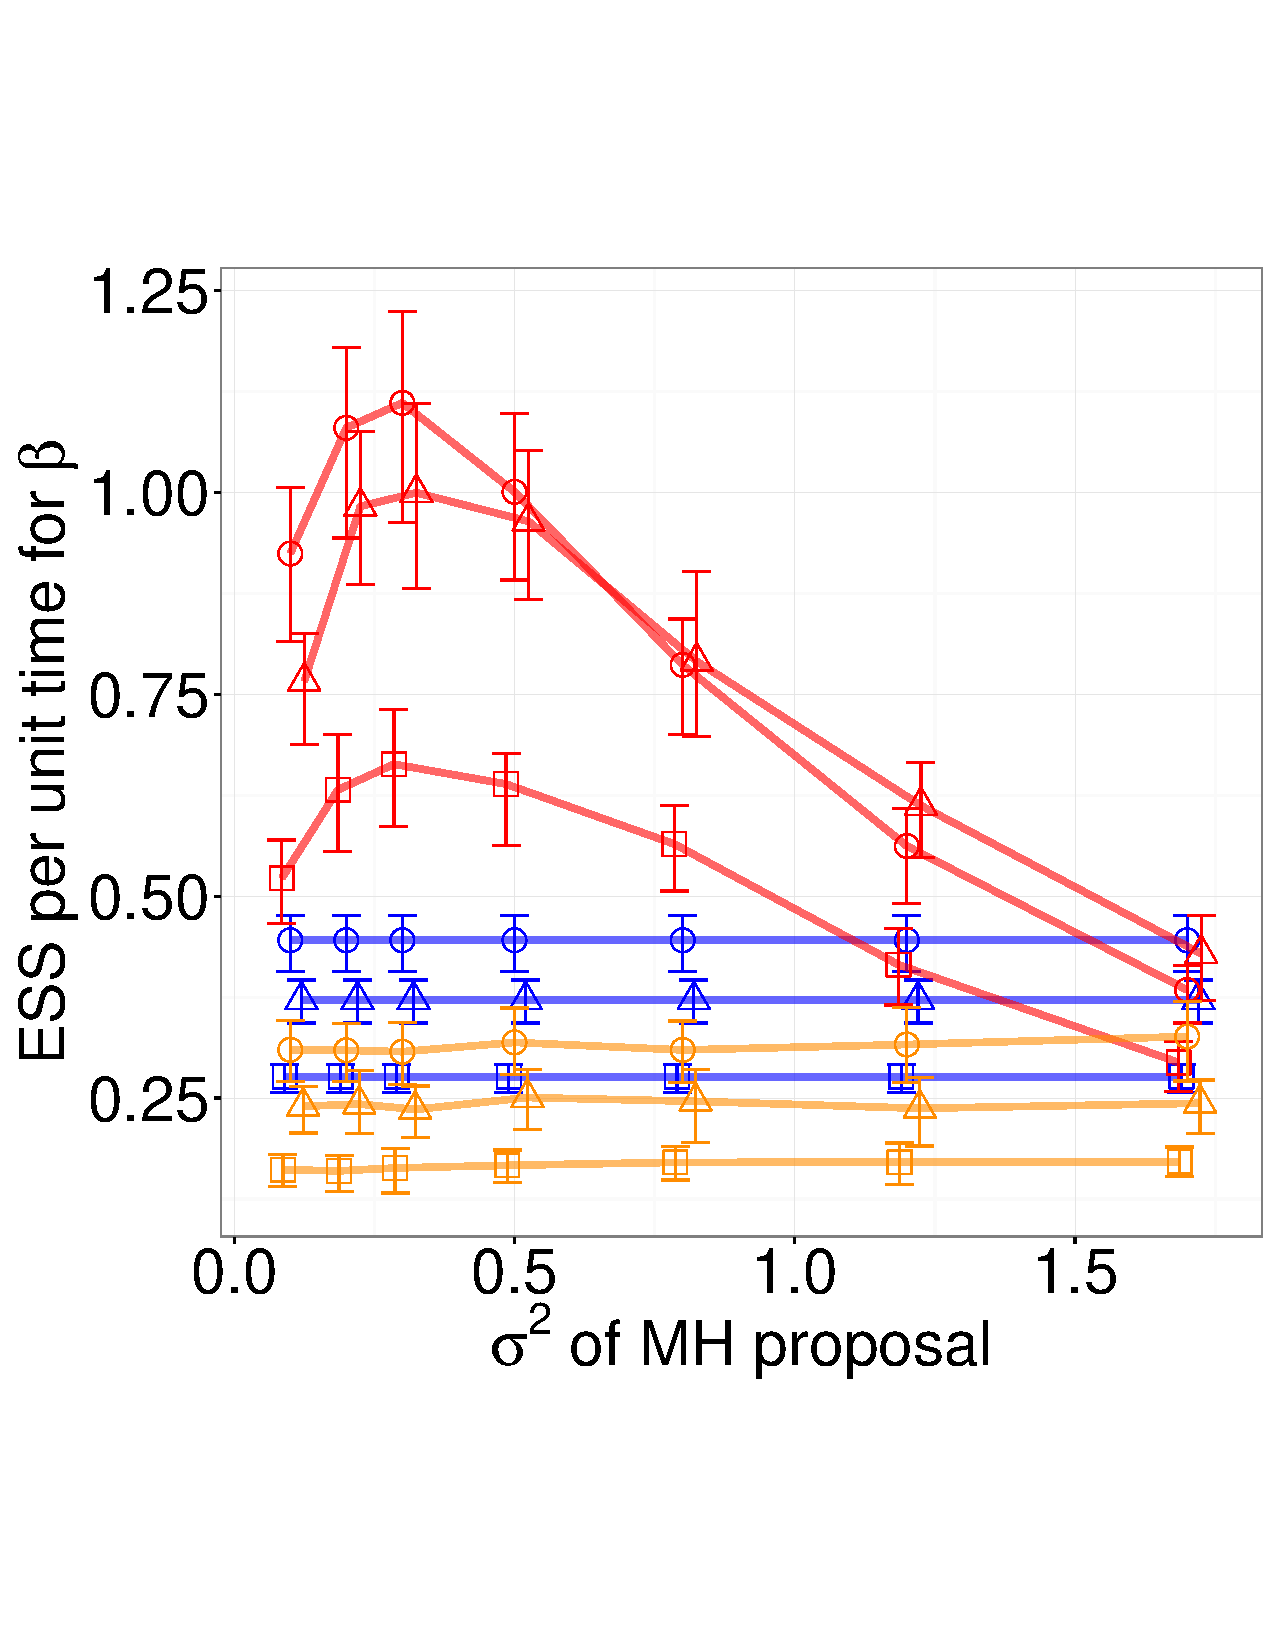
\includegraphics [width=0.44\textwidth, angle=0]{figs/pc_5_beta.pdf}
  \end{minipage}
  \begin{minipage}[!hp]{0.33\linewidth}
    \caption{ESS/sec for the time-inhomogeneous immigration model, with 
      dimension 5. (Left, right) are $(\alpha, \beta)$. Red, yellow and blue curves are the symmetrized MH,
  \naive\ MH, and Gibbs algorithm.}
     \label{fig:ESS_pc_5}
  \end{minipage}
% \centering
% \begin{minipage}[!hp]{0.64\linewidth}
%   \hspace{.15in}
%   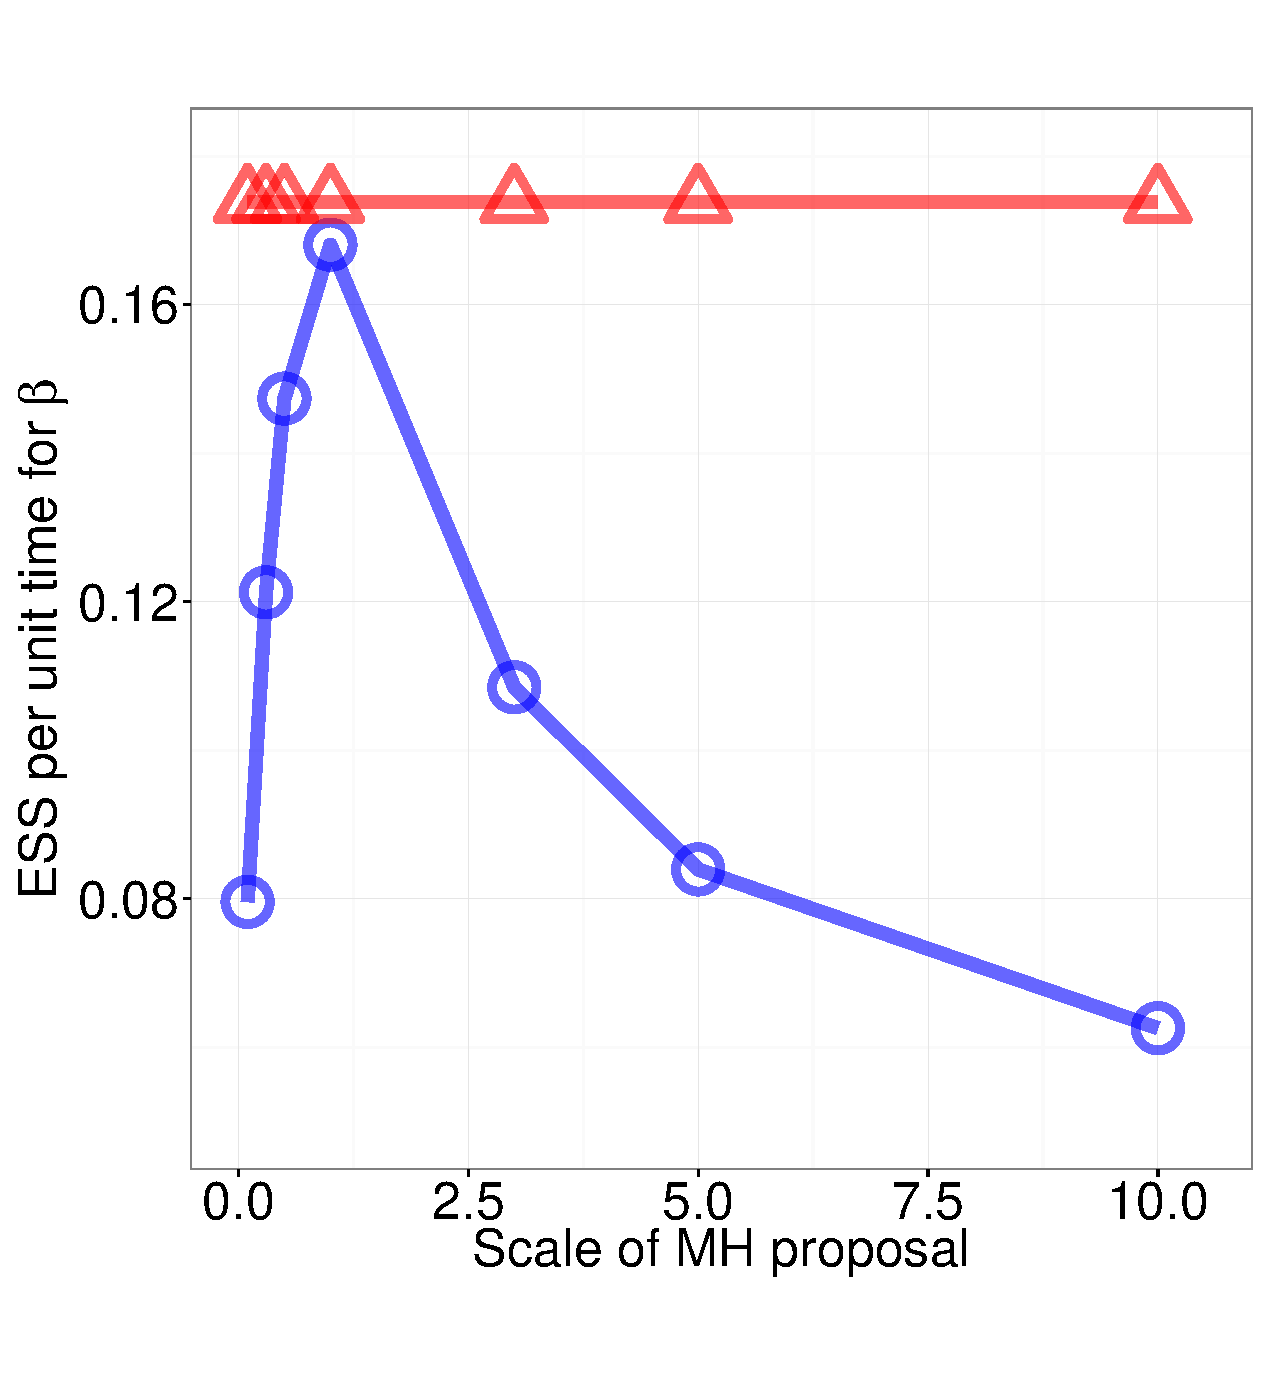
\includegraphics [width=0.44\textwidth, angle=0]{figs/ECOLI_beta.pdf}
%   \hspace{.15in}
%   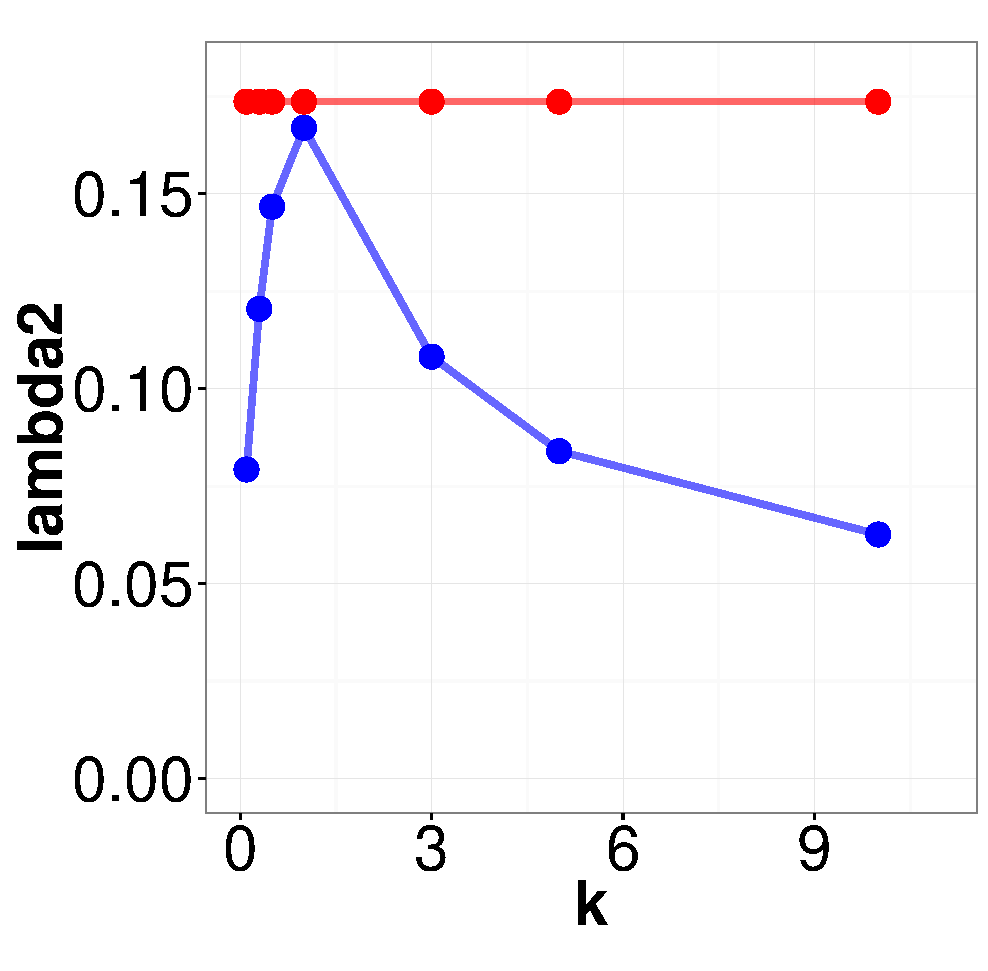
\includegraphics [width=0.44\textwidth, angle=0]{figs/ECOLI_l2.pdf}
% \end{minipage}
%   \hspace{-.3in}
% \begin{minipage}[!hp]{0.05\linewidth}
%   \hspace{0in}
%   \end{minipage}
% \begin{minipage}[!hp]{0.33\linewidth}
%   \caption{ESS/sec for EColi data. The left column is for $\beta$, and the 
%   right is for $\lambda_2$. Red and blue curves are Gibbs algorithm and the symmetrized MH.}
% \end{minipage}
%    \label{fig:ECOLI_beta_l2}
  \end{figure}
